%%
%% Copyright 2024 OXFORD UNIVERSITY PRESS
%%
%% ---------------------------------------------
%%
%% It may be distributed under the conditions of the LaTeX Project Public
%% License, either version 1.2 of this license or (at your option) any
%% later version.  The latest version of this license is in
%%    http://www.latex-project.org/lppl.txt
%% and version 1.2 or later is part of all distributions of LaTeX
%% version 1999/12/01 or later.
%%
%% The list of all files belonging to the 'oup-authoring-template Bundle' is
%% given in the file `manifest.txt'.
%%
%% Template article for OXFORD UNIVERSITY PRESS's document class `oup-authoring-template'
%% with bibliographic references
%%

\documentclass[numsec,webpdf,modern,medium,namedate]{oup-authoring-template}
\onecolumn

%\usepackage{showframe}

\graphicspath{{Figures/}}

% line numbers
%\usepackage[mathlines, switch]{lineno}
%\usepackage[right]{lineno}

% Re-define OUP theorem styles with reduced spaceabove/below before declaring
% \newtheorem environments.  The cls defaults are 12pt; under doublespacing the
% preceding blank line already contributes ~24 pt of vertical space, so the
% extra 12 pt creates a visually jarring double-gap.  Reducing to 3 pt keeps
% environments visually distinct without the excess white space.
\makeatletter
\newtheoremstyle{thmstyleone}%
  {3pt plus1pt minus1pt}% space above (was 12pt)
  {3pt plus1pt minus1pt}% space below
  {\normalfont\itshape}%
  {0pt}%
  {\bfseries}%
  {}%
  {.5em}%
  {\thmname{#1}\thmnumber{\@ifnotempty{#1}{ }\@upn{#2}}\thmnote{ {\the\thm@notefont(#3)}}}%
\newtheoremstyle{thmstyletwo}%
  {3pt plus1pt minus1pt}%
  {3pt plus1pt minus1pt}%
  {\itshape}%
  {0pt}%
  {\normalfont}%
  {}%
  {.5em}%
  {\thmname{#1}\thmnumber{\@ifnotempty{#1}{ }{#2}}\thmnote{ {\the\thm@notefont(#3)}}}%
\newtheoremstyle{thmstylethree}%
  {3pt plus1pt minus1pt}%
  {3pt plus1pt minus1pt}%
  {\normalfont}%
  {0pt}%
  {\bfseries}%
  {}%
  {.5em}%
  {\thmname{#1}\thmnumber{\@ifnotempty{#1}{ }\@upn{#2}}\thmnote{ {\the\thm@notefont(#3)}}}%
\makeatother
\theoremstyle{thmstyleone}%
\newtheorem{theorem}{Theorem}%  meant for continuous numbers
%%\newtheorem{theorem}{Theorem}[section]% meant for sectionwise numbers
%% optional argument [theorem] produces theorem numbering sequence instead of independent numbers for Proposition
% \newtheorem{proposition}[theorem]{Proposition}%
\newtheorem{proposition}{Proposition}
\newtheorem{assumption}{Assumption}% to get separate numbers for theorem and proposition etc.
\theoremstyle{thmstyletwo}%
\newtheorem{example}{Example}%
\newtheorem{remark}{Remark}%
\theoremstyle{thmstylethree}%
\newtheorem{definition}{Definition}
\usepackage[doublespacing]{setspace}
% Prevent doublespacing from multiplying display-math skips.
\setdisplayskipstretch{1.0}
% Keep list topsep reasonable inside theorem environments.
\usepackage{etoolbox}
\AtBeginDocument{%
  \setlength{\topsep}{6pt plus 1pt minus 1pt}%
}
% Reduce section/subsection pre-skip to compensate for doublespacing.
% The cls defaults (16pt / 11pt) stack on top of the doubled baseline (~24pt)
% from the blank line before each heading, producing an excessive gap.
% Reducing to 4pt gives a total of ~28pt (a little over one doublespaced line).
\makeatletter
\def\section{%
  \@startsection{section}{1}{\z@}
  {-4\p@ plus -2\p@}{\if@traditional\if@large.4\p@\else\if@medium6.5\p@\else4\p@\fi\fi\else\if@contemporary5\p@\else4\p@\fi\fi}
  {\reset@font\raggedright\secsize}}
\def\subsection{%
  \@startsection{subsection}{2}{\z@}
  {-4\p@ plus -2\p@}{\if@traditional.4\p@\else2\p@\fi}
  {\reset@font\raggedright\subsecsize}}
\makeatother
\usepackage[fontsize=12pt]{fontsize}
\usepackage{xcolor}
\usepackage{hyperref}

\hypersetup{
    colorlinks=true,
    linkcolor=blue,      % internal links (sections, equations, figures)
    citecolor=blue,      % citation links
    urlcolor=blue        % URLs
}
%%%%%%% CUSTOM PACKAGES %%%%%%%%%%
\DeclareMathOperator*{\argmax}{arg\,max}
\DeclareMathOperator*{\argmin}{arg\,min}
\newcommand{\noi}{\noindent}
\newcommand{\norm}[1]{\left\lVert #1 \right\rVert}
\newcommand{\nlim}{\xrightarrow[]{n \to \infty}}
\newcommand{\pnlim}{\xrightarrow[n \to \infty]{P}}
\newcommand{\klim}{\xrightarrow[]{k \to \infty}}
\newcommand{\aslim}{\xrightarrow[n \to \infty]{a.s.}}
\newcommand{\dnlim}{\xrightarrow[n \to \infty]{d}}
\newcommand{\lnlim}{\xrightarrow[n \to \infty]{L_2}}
\newcommand{\bmu}{\boldsymbol{\mu}}
\newcommand{\tr}{\mathrm{tr}}
\newcommand{\calB}{\mathcal{B}}
\newcommand{\calC}{\mathcal{C}}
\newcommand{\calD}{\mathcal{D}}
\newcommand{\calL}{\mathcal{L}}
\newcommand{\calP}{\mathcal{P}}
\newcommand{\calH}{\mathcal{H}}
\newcommand{\calHP}{\mathcal{P}}
\newcommand{\calI}{\mathcal{I}}
\newcommand{\calQ}{\mathcal{Q}}
\newcommand{\calN}{\mathcal{N}}
\newcommand{\R}{\mathbb{R}}
\newcommand{\N}{\mathbb{N}}
\newcommand{\Q}{\mathbb{Q}}
\newcommand{\bigo}{\mathcal{O}}
\newcommand{\smallo}{o}
\newcommand{\Z}{\mathbb{Z}}
\newcommand{\bdn}{\bar{d}_n}
\newcommand{\bE}{\mathbf{E}}
\newcommand{\bW}{\boldsymbol{W}}
\newcommand{\bX}{\boldsymbol{X}}
\newcommand{\bR}{\mathbf{R}}
\newcommand{\bpix}{\boldsymbol{\pi}_X}
\newcommand{\bpis}{\boldsymbol{\pi}_S}
\newcommand{\bPix}{\boldsymbol{\Pi}_X}
\newcommand{\bPis}{\boldsymbol{\Pi}_S}
\newcommand{\bPi}{\boldsymbol{\Pi}}
\newcommand{\bpi}{\boldsymbol{\pi}}
\newcommand{\hatpi}{\widehat{\boldsymbol{\pi}}}
\newcommand{\hatPi}{\widehat{\boldsymbol{\Pi}}}
\newcommand{\hatPix}{\widehat{\boldsymbol{\Pi}}_x}
\newcommand{\hatPis}{\widehat{\boldsymbol{\Pi}}_s}
\newcommand{\bPisx}{\boldsymbol{\Pi}_s\boldsymbol{\Pi}_x}
\newcommand{\delnu}{\Delta\nu}
\newcommand{\bY}{\boldsymbol{Y}}
\newcommand{\bM}{\mathbf{M}}
\newcommand{\bB}{\mathbf{B}}
\newcommand{\bK}{\mathbf{K}}
\newcommand{\by}{\boldsymbol{y}}
\newcommand{\bu}{\boldsymbol{u}}
\newcommand{\bz}{\boldsymbol{z}}
\newcommand{\bzet}{\boldsymbol{\zeta}}
\newcommand{\bGam}{\boldsymbol{\Gamma}}
\newcommand{\bQ}{\boldsymbol{Q}}
\newcommand{\bh}{\boldsymbol{h}}
\newcommand{\bD}{\boldsymbol{D}}
\newcommand{\bT}{\mathbf{T}}
\newcommand{\br}{\boldsymbol{r}}
\newcommand{\bV}{\mathbf{V}}
\newcommand{\bS}{\boldsymbol{S}}
\newcommand{\ba}{\boldsymbol{a}}
\newcommand{\balp}{\boldsymbol{\alpha}}
\newcommand{\snr}{\mathrm{SNR}}
\newcommand{\bdiag}{\mathrm{bdiag}}
\newcommand{\bDel}{\boldsymbol{\Delta}}
\newcommand{\bA}{\mathbf{A}}
\newcommand{\boldW}{\mathbb{W}}
\newcommand{\boldY}{\mathbb{Y}}
\newcommand{\boldX}{\mathbb{X}}
\newcommand{\boldM}{\mathbb{M}}
\newcommand{\boldV}{\mathbb{V}}
\newcommand{\bZ}{\boldsymbol{Z}}
\newcommand{\bU}{\boldsymbol{U}}
\newcommand{\bL}{\boldsymbol{L}}
\newcommand{\bP}{\mathbf{P}}
\newcommand{\bLam}{\boldsymbol{\Lambda}}
\newcommand{\blam}{\boldsymbol{\lambda}}
\newcommand{\bx}{\boldsymbol{x}}
\newcommand{\bI}{\mathbf{I}}
\newcommand{\beps}{\boldsymbol{\epsilon}}
\newcommand{\bet}{\boldsymbol{\eta}}
\newcommand{\bSig}{\boldsymbol{\Sigma}}
\newcommand{\Siginv}{\boldsymbol{\Sigma}^{-1}}
\newcommand{\ra}{\rightarrow}
\newcommand{\la}{\leftarrow}
\newcommand{\fld}{\mathcal{F}}
\newcommand{\Cov}{\text{Cov}\,}
\newcommand{\bard}{\bdn}
\newcommand{\pr}{\mathbb{P}}
\newcommand{\E}{\mathbb{E}}
\newcommand{\colsp}{\mathscr{C}}
% \newtheorem{theorem}{Theorem}
% \newtheorem{corollary}{Corollary}
% \newtheorem{lemma}{Lemma}
% \newtheorem{proposition}{Proposition}
% \newtheorem{posterior}{Posterior}
% \newtheorem{assumption}{Assumption}
% \theoremstyle{definition}
% \newtheorem{definition}{Definition}
% \newtheorem{remark}{Remark}
% \newtheorem{example}{Example}
% \newtheorem{conjecture}{Conjecture}
\newcommand{\Tau}{\mathcal{T}}
\newcommand{\bSigma}{{\boldsymbol{\Sigma}}}
\newcommand{\transpose}{^\top}
% %%%%%%%%%%%%%%%%%%%%%%%%%%%%%%%%%%%%%%%%%

\newcommand{\rough}{\underset{\sim}{<}}
\newcommand{\bH}{\boldsymbol{H}}
\newcommand{\bep}{\boldsymbol{\epsilon}}
\newcommand{\hbn}{\hat{\beta}_n}
\newcommand{\ets}{\eta^{*}}
% \newcommand{\BM}{\mathbf{M}}
\newcommand{\bTh}{\boldsymbol{\Theta}}
\newcommand{\bth}{\boldsymbol{\theta}}
\newcommand{\bets}{\boldsymbol{\eta}^{*}}
\newcommand{\betap}{\beta^{'}}
\newcommand{\ystbp}{Y^{*}_{\betap}}
\newcommand{\bystbp}{\boldsymbol{Y}^{*}_{\betap}}
\newcommand{\bystb}{\boldsymbol{Y}^{*}_{\beta}}
\newcommand{\Xstar}{X^{*}}
\newcommand{\bXstar}{\boldsymbol{X}^{*}}
\newcommand{\bs}{\boldsymbol{s}}
\newcommand{\tilX}{\widetilde{\boldsymbol{X}}}
\newcommand{\tilY}{\widetilde{\boldsymbol{Y}}}
\newcommand{\tbH}{\boldsymbol{H}^{'}}
\newcommand{\tbh}{\boldsymbol{h}^{'}}
\newcommand{\bdel}{\boldsymbol{\delta}}
\newcommand{\bnu}{\boldsymbol{\nu}}
\newcommand{\bgam}{\boldsymbol{\gamma}}
\newcommand{\bzero}{\boldsymbol{0}}
\newcommand{\Prob}{\mathbb{P}}
\newcommand{\Pst}{\mathbb{P}^{*}}
\newcommand{\betahat}{\hat{\beta}}

\newcommand{\hly}[1]{\colorbox{yellow}{#1}}
\newcommand{\iid}{\stackrel{\mathclap{\normalfont\tiny\mbox{iid}}}{\sim}}
\newcommand{\given}{\,|\,}
\newcommand{\biggiven}{\,\middle|\,}
\newcommand{\V}{\mathbb{V}}
\newcommand{\defeq}{\vcentcolon=}
\newcommand{\DY}{\mathrm{DY}}
\newcommand{\CM}{\mathrm{CM}}
\newcommand{\GCM}{\mathrm{GCM}}
\newcommand{\CMc}{\mathrm{CM_c}}
\newcommand{\GCMc}{\mathrm{GCM_c}}
\newcommand{\Cor}{\mathrm{Cor}}





% \newtheorem{theorem}{Theorem}
\newtheorem{corollary}{Corollary}
\newtheorem{lemma}{Lemma}
% \newtheorem{proposition}{Proposition}
% \newtheorem{posterior}{Posterior}
% \newtheorem{assumption}{Assumption}
% \newtheorem{definition}{Definition}
% \newtheorem{remark}{Remark}
% \newtheorem{example}{Example}
% \newtheorem{conjecture}{Conjecture}
\usepackage{mathtools}
\usepackage{nicefrac} 
\usepackage{hyperref}
\usepackage{xcolor}
\usepackage{algorithm}
\usepackage{algpseudocode}
\definecolor{darkgreen}{RGB}{0,100,0}
\newcommand{\pink}[1]{{\leavevmode\color{magenta}{#1}}}
\newcommand{\green}[1]{{\leavevmode\color{darkgreen}{#1}}}
\newcommand{\red}[1]{{\leavevmode\color{red}{#1}}}


\usepackage{xr-hyper}
\externaldocument{doubly_unlinked_supplement}

\begin{document}

\journaltitle{Preprint}
\DOI{DOI HERE}
\copyrightyear{XXXX}
\pubyear{XXXX}
\access{Advance Access Publication Date: Day Month Year}
\appnotes{Original article}

\firstpage{1}

%\subtitle{Subject Section}

\title[Doubly-Unlinked Regression]{Doubly-Unlinked Regression for Dependent Data}

\author[1]{Anik Burman}
\author[2]{Sayantan Choudhury}
% \author[3]{}
% \author[3]{Fourth Author}
\author[3,$\ast$]{Debangan Dey\ORCID{0000-0002-2579-5693}}

\authormark{Burman et al.}

\address[1]{\orgdiv{Department of Biostatistics}, \orgname{Johns Hopkins University}, \orgaddress{\street{615 N Wolfe St}, \postcode{21205}, \state{Maryland}, \country{USA}}}
\address[2]{\orgdiv{Department of Statistics and Data Science}, \orgname{Mohamed bin Zayed University of Artificial Intelligence}, \orgaddress{\postcode{SE4505}, \state{Abu Dhabi}, \country{UAE}}}
\address[3]{\orgdiv{Department of Statistics}, \orgname{Texas A\&M University}, \orgaddress{\street{155 Ireland Street},\state{Texas}, \country{USA}}}

\corresp[$\ast$]{Address for correspondence. Debangan Dey, Texas A\&M University, College Station, TX, 77843. Email: \href{Email:debangan@tamu.edu}{debangan@tamu.edu}}

\received{Date}{0}{Year}
\revised{Date}{0}{Year}
\accepted{Date}{0}{Year}

%\editor{Associate Editor: Name}

%% (old draft abstract removed -- real abstract is in bstract{} below)

\abstract{
% Abstracts must be able to stand alone and so cannot contain citations to
% the paper's references, equations, etc. An abstract must consist of a single
% paragraph and be concise. Because of online formatting, abstracts must appear
% as plain as possible.
Modern spatial and temporal datasets often violate the standard assumption that covariates, responses, and their underlying domain are correctly aligned. In practice, correspondence may fail in two ways: the covariate--response link may be broken when exposures and outcomes are observed without their correct pairing, and the response--domain link may be broken when responses are detached from the spatial or temporal structure inducing their dependence. While existing work studies unlinked regression with a single missing correspondence under independent observations, the simultaneous loss of both correspondences in dependent data has not been systematically studied. We introduce the doubly-unlinked regression model, in which covariates and latent domain processes are observed through two unknown permutations that break the covariate--response and response--domain links. We characterize signal-to-noise regimes governing recovery of the regression parameter and the latent permutations, and show that consistent estimation of the regression effect can be achieved under strictly weaker signal conditions than those required for exact permutation recovery. Consequently, valid inference on the regression signal can remain feasible even when the underlying correspondences cannot be recovered. We develop REPAIR, a variational Bayes method for joint estimation of the regression parameter, latent permutations, and parameters governing the covariance structure. Simulations and an application to a real-world dataset illustrate the empirical performance of the proposed approach.
}
\keywords{
% keyword1, Keyword2, Keyword3, Keyword4
Shuffled regression, Dependent data, Spatial data, Exponential covariance, Permutation inference, Variational Bayes
}

\maketitle
\section{Introduction}\label{sec-intro}

Modern spatial and temporal datasets are typically analyzed under the assumption
that covariates, responses, and their underlying spatial or temporal domain are
correctly aligned.
In practice, however, these correspondences may be partially or completely
missing.
Two distinct failures can occur.
The first is a broken covariate--response link: in survey-based epidemiological
studies, exposure records, and health outcomes are often drawn from separate
registries and linked imperfectly, leaving the covariate--response pairing
uncertain \citep{lahiri2005regression}; in genomics, sample mix-ups during
high-throughput sequencing attaches gene expression profiles to the wrong
phenotypic outcomes \citep{westra2011mixupmapper}.
The second is a broken response--domain link: dissociation-based transcriptomics
protocols lyse individual cells from tissue to sequence their transcriptomes,
discarding spatial positional identity in the process \citep{nitzan2019charting};
analogous ordering failures arise in pseudo-time inference
\citep{gu2022bayesian}, seriation in archaeology \citep{banning2020seriation},
and spike sorting in neural arrays \citep{rossant2016spike}. 
Both failures also arise deliberately when data are released under geoprivacy
constraints that obscure spatial locations or covariate pairings to protect
individual identities \citep{lin2023geo, cassa2008re}.
These settings raise a fundamental question about whether recovering the domain correspondence is necessary for inferring the underlying regression signal, or whether valid inference can proceed even when the permutations linking covariates, responses, and domain structure remain unknown. In this paper, we develop theory and methods to address both settings.

Let $\bX=(X(s_1),\dots,X(s_n))^\top$ denote the covariate vector, let
$\bY=(Y(s_1),\dots,Y(s_n))^\top$ denote the response vector, and let
$\bW=(W(s_1),\dots,W(s_n))^\top$ denote a latent stochastic process at
sampled domain points $s_1,\dots,s_n$.
We consider the joint loss of correspondence through the data generating process (DGP)
\begin{equation}
\label{eq:dgp}
\bY=\bPix \bX \beta+\bPis \bW+\beps,
\end{equation}
where $\bPix$ and $\bPis$ are unknown permutation matrices.
The permutation $\bPix$ breaks the covariate--response link while $\bPis$
breaks the response--domain link through which dependence is induced.
The joint problem is not a superposition of two known single-link problems.
Recovery of $\bPix$ alone is polynomial-time tractable in iid settings
\citep{zhang2020optimal}, but recovery of $\bPis$ leads to a quadratic
assignment problem that is NP-hard \citep{loiola2007}; their coupling through
$\beta$ and the structure of the process covariance make the combined
problem harder.
More fundamentally, the latent dependence alters the information geometry in a
way that creates distinct recovery regimes for $\beta$ and for $(\bPix,\bPis)$,
a phenomenon not explored in the existing iid shuffled regression literature.

\begin{figure}[!ht]
    \centering
    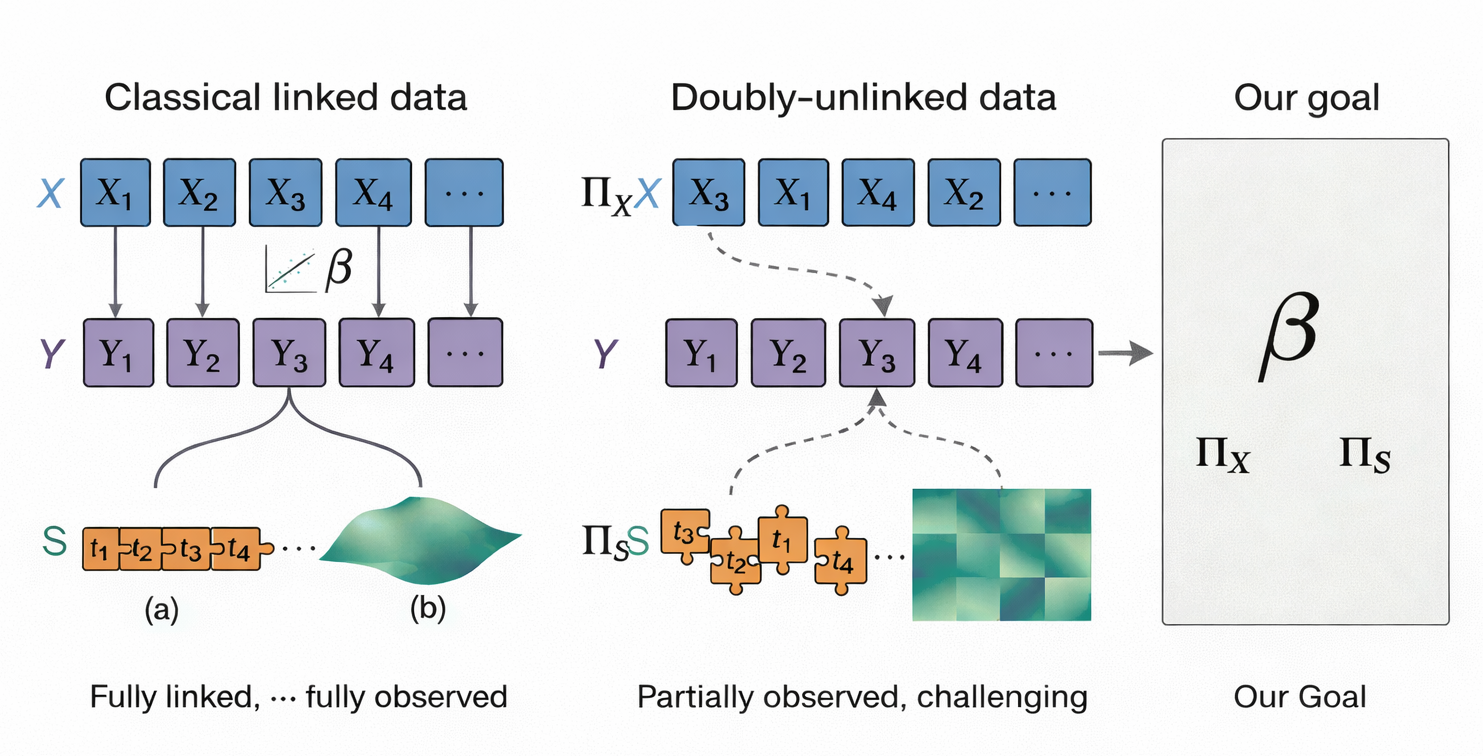
\includegraphics[width=\textwidth]{Figures/unlinked_regression_explanation.png}
    \caption{Schematic illustration of the doubly-unlinked regression setting. The left panel shows the classical linked-data setting with aligned exposures, outcomes, and domain variables and regression effect $\beta$. The middle panel depicts the doubly-unlinked setting, where exposures and domain variables are observed after unknown permutations. The primary inferential target is $\beta$, while recovery of $\bpix$ and $\bpis$ is secondary.}
    \label{fig:unlinked-reg-illustration}
\end{figure}

The theory of unlinked regression under iid observations is now well-developed.
Foundational work established identifiability and recovery limits:
\citet{unnikrishnan2015unlabeled} showed that the permutation is generically
identifiable from unlabeled measurements, and \citet{pananjady2017linear}
characterised a sharp signal-to-noise threshold below which permutation
recovery is information-theoretically impossible regardless of computational
budget.
Subsequent work derived statistically and computationally efficient joint
estimators \citep{zhang2020optimal}, polynomial-time convex relaxations
\citep{slawski2019, pananjady2018}, and extensions to spectral, graph-based,
and optimal transport formulations
\citep{hsu2017, liu2025shuffled, liu2024blind, beuthner2021data, Slawski2024a,
Wang2023, durot2024minimax, Fabrizi2025}.
All of this work assumes iid observations and a single broken link; none
addresses the spatial or temporal dependence that characterises the
applications motivating this paper.
The doubly-unlinked model studied here involves both failures simultaneously
under structured dependence, and produces a qualitatively new phenomenon: the
threshold governing permutation recovery and the condition for consistent
$\beta$ estimation are strictly different, a separation with no counterpart in
the existing iid shuffled regression literature.

This paper makes three contributions.
First, we introduce the doubly-unlinked regression setup \eqref{eq:dgp} as the
first systematic framework for regression under simultaneous covariate--response
and response--domain correspondence failures in dependent data, and provide a
theoretical characterisation of the signal-to-noise conditions governing
permutation and regression recovery.
The central finding is a separation: the SNR condition sufficient for
consistent estimation of $\beta$ is strictly weaker than the condition
sufficient for exact permutation recovery, so that valid regression inference
remains feasible in signal regimes where permutation recovery is not guaranteed.
This separation has a natural implication for spatial data release.
Most spatial regression models already adopt a Gaussian process prior, under
which individual locations are treated as samples from a smooth latent surface
rather than as fixed identities.
The inferential target is then the population-level exposure effect $\beta$,
not individual-level spatial attribution.
Our results show that a structured scrambling of both covariate assignments and
spatial coordinates can protect individual-level correspondence while leaving
$\beta$ consistently estimable, pointing to a class of privacy mechanisms
distinct from spatial aggregation or noise addition.
Second, we develop \textsc{repair} (\textbf{RE}gression with \textbf{P}ermutation
\textbf{A}lignment via Variational \textbf{I}nfe\textbf{R}ence), a variational
Bayes algorithm for joint inference on $\beta$, the two latent permutations
matrices, and the covariance parameters of the latent process, built on a
block-structured permutation model that captures localized scrambling.
Third, simulation studies and an applied analysis on the Meuse soil dataset
confirm that \textsc{repair} recovers $\beta$ accurately across a range of
settings, with near-oracle performance at high SNR; the exposure permutation
$\bpix$ is reliably recovered across settings, while recovery of the spatial
permutation $\bpis$ improves as the block structure becomes finer.

The remainder of the paper is organized as follows.
Section~\ref{sec:dgp} introduces the DGP and formal
assumptions.
Section~\ref{sec:theory} presents the main theoretical results.
Section~\ref{sec:vb} develops \textsc{repair}.
Section~\ref{sec:simulation} investigates finite-sample performance,
Section~\ref{sec:data} presents the applied analysis, and
Section~\ref{sec:discussion} concludes.

\section{Background and Problem Setup}\label{sec:dgp}
\textbf{Notation.}
We use the standard order notation $\bigo(\cdot)$ and $\Omega(\cdot)$ throughout. For two nonnegative sequences $a_n$ and $b_n$, we write $a_n=\bigo(b_n)$ if there exist constants $C>0$ and $N$ such that $a_n\le C b_n$ for all $n\ge N$, and $a_n=\Omega(b_n)$ if there exist constants $c>0$ and $N$ such that $a_n\ge c b_n$ for all $n\ge N$. For a vector $\bx\in\R^d$, $\|\bx\|_2$ denotes the Euclidean norm. For a matrix $\bA$, $\|\bA\|_2$ denotes the spectral norm unless stated otherwise.

\textbf{Formal Problem Setup.} We consider the DGP \eqref{eq:dgp} over a latent domain $\calD\subset\R^k$. Let $\{s_i\}_{i=1}^n\subset\calD$ denote observed domain points, and let $\bW$ 
be a mean-zero latent process with covariance matrix $\bSig^\ast$. It represents structured dependence induced by the domain $\calD$. Such dependence is ubiquitous in time-series analysis, spatial statistics, longitudinal studies, sensor networks, and manifold-based biological data. Even if individual-level correspondences are scrambled, the covariance structure induced by $W(s_i)$ reflects the geometry or ordering of the underlying domain. Our primary inferential objective is estimation of $\beta$, with recovery of the permutations treated as a secondary objective when feasible. We begin by stating the assumptions imposed on the DGP in \eqref{eq:dgp}. Additional structural restrictions used to make inference tractable will be introduced subsequently.
% \vspace{-1.2ex}
\begin{assumption}[Data Generation Assumption]\label{assume:dgp}
We assume that the data generation process satisfies:
\begin{itemize}
    \item The exposure vector $\bX \sim \calN_n\left(\bzero, \sigma_X^2 \bI_n \right)$.
    \item $W(s_i)$ is a realization from $\mathcal{GP}(0, C(\cdot,\cdot))$ where the covariance function $C(\cdot,\cdot)$ belongs to a known isotropic class indexed by parameters $\bGam = \left(\gamma_1, \cdots, \gamma_c\right)^\top$.
    \item $\bX$ is independent of $\bW$, i.e., there is no latent endogeneity.
    \item The random error vector $\beps \sim \calN_n \left(\bzero, \tau^2 \bI_n\right)$ is independent of $\bX$ and $\bW$.
\end{itemize}
\end{assumption}
Under Assumption~\ref{assume:dgp}, the random effects vector observed at the $n$ domain indices $\bS=(s_1,\dots,s_n)^{\top}$ satisfies $\bW \sim \calN_n(\bzero, \bSig^\ast)$ where $\bSig^\ast = \sigma^2\bR_{\bth^\ast}$ and $\bR_{\bth^\ast}$ is the corresponding correlation matrix induced by $C(\cdot,\cdot)$ evaluated at $\bS$, parametrised by $\bGam = (\sigma^2,\bth^\ast)$. Marginalizing over $\bW$ yields $\bY|\bX \sim  \calN_n\left(\bPix\bX\beta, \bPis\left(\bSig^\ast + \tau^2 \bI_n\right)\bPis^\top\right)$. Defining $\bSig = \bSig^\ast + \tau^2 \bI_n$, the conditional covariance of $\bY$ is $\bPis\bSig\bPis^\top$.

Because the latent process $\bW$ is not observed, direct inference on $\bPis$ is generally infeasible. For theoretical purposes, it is convenient to reparameterize $(\bPis,\bPix)$ through the one-to-one transformation $(\bPis,\bPix)\mapsto (\bPi_1,\bPi_2)$ defined by $\bPi_1=\bPis^\top \bPix$ and $\bPi_2=\bPis^\top$. We emphasize that this reparameterization is introduced only to facilitate analysis; the methodological development will be presented in the original parametrization. Left-multiplying \eqref{eq:dgp} by $\bPi_2$ gives $\bPi_2 \bY = \bPi_1 \bX \beta + \bW^\ast$, where $\bW^\ast \sim \calN_n(\bzero,\bSig)$. This representation recasts the problem as a Generalized Least Squares (GLS) version of shuffled regression under correlated errors.
Assuming that $\bSig$ is known, define $\bTh \coloneqq \left(\bPi_1, \bPi_2, \beta \right)$ and consider the GLS loss function
\begin{equation}\label{eq:loss-fn}
    \begin{split}
            \mathcal{L}(\bTh)  \coloneqq & \left\|\widetilde{\bY}_{\bPi_2} - \widetilde{\bX}_{\bPi_1}\beta\right\|^2_2 \\
     = & \underbrace{\left\|\bP_{\bPi_1,X}^\perp\widetilde{\bY}_{\bPi_2}\right\|^2_2}_{\calL_1(\bTh)} + \underbrace{\left\|\bP_{\bPi_1,X}\widetilde{\bY}_{\bPi_2} - \widetilde{\bX}_{\bPi_1}\beta\right\|^2_2}_{\calL_2(\bTh)}, 
    \end{split}
\end{equation}
where $\widetilde{\bX}_{\bPi_1} \coloneqq {\bSig}^{- \nicefrac{1}{2}}\bPi_1 \bX$, $\widetilde{\bY}_{\bPi_2} \coloneqq {\bSig}^{-\nicefrac{1}{2}}\bPi_2 \bY$, and $\bP_{\bPi_1,X}$ is the projection matrix onto the column space of $\widetilde{\bX}_{\bPi_1}$ with $\bP_{\bPi_1,X}^\perp\coloneq \bI_n - \bP_{\bPi_1,X}$.
We need to minimize the loss function \eqref{eq:loss-fn} in order to estimate $\bTh$.

\textbf{Block Permutation Structure.}
The fully unrestricted permutation model allows $(n!)^2$ possible pairs $(\bPi_1,\bPi_2)$, rendering both theoretical characterization and computation intractable for even moderate $n$. Moreover, in many practical settings, scrambling mechanisms are not globally arbitrary but instead exhibit localized structure. To reflect this and to obtain a statistically meaningful intermediate regime between complete correspondence and fully adversarial permutations, we impose a structured restriction on $\bPi_1$ and $\bPi_2$.

For $n$ sampled domain indices, we partition them into $B$ blocks of size $K$, so that $n = KB$. Within each block, exposure values and domain indices may be permuted, but no permutation occurs across blocks. This restriction models localized scrambling mechanisms such as batching, windowed anonymization, temporal shuffling within short time segments, or partial reordering within contiguous domain neighborhoods. In such settings, coarse-scale ordering across blocks is preserved, while fine-scale correspondences within blocks are obscured.

From a statistical perspective, the block structure creates an intermediate inferential regime: the latent dependence induced by $W(s_i)$ continues to operate across blocks, preserving large-scale covariance structure, while local permutations disrupt short-range alignment between $\bX$ and $\bY$. This separation allows us to study whether regression recovery can exploit global dependence even when local correspondences are scrambled. The block model, therefore, isolates the interaction between dependence and permutation noise without requiring recovery over the full combinatorial space.

We further assume that, for the two $K \times K$ permutation matrices $\bpi_1 \coloneqq \bpix^\top \bpis$ and $\bpi_2 \coloneqq \bpis^\top$, the corresponding full permutation matrices of size $n = KB$ satisfy
$\bPi_u = \operatorname{bdiag}(\bpi_u)$ for $ u = 1,2$ where $\operatorname{bdiag}(\bA)$ denotes block diagonal matrix with the same $\bA$ repeated. Thus, the same within-block permutation is repeated across all $B$ blocks. This assumption is convenient both analytically and computationally, as it imposes a simple structure while still allowing for local scrambling within each block. It is also natural in settings where observations are perturbed according to a common mechanism across blocks; for example, when data are masked prior to release, the same permutation rule may be applied repeatedly within each block. Under this specification, there is a correspondence between $\bPi_X$ and $\bPi_S$ with the corresponding block matrices $\bpix$ and $\bpis$. Similarly any estimate $\hatPi_u$ can be represented as $\bdiag(\hatpi_u)$. For Hamming distance $d_H$ between the identity  matrix $\bI_K$ and $\bpi_u$ equal to $d_H(\bI_K,\bpi_u) = k_u$, we have $d_H(\bI_n,\bPi_u) = h_u = k_uB$, and analogous definitions apply to $\hatpi_u$ and $\hatPi_u$ with corresponding $\hat{k}_u$. We will use these notations throughout.

Under Assumption~\ref{assume:dgp}, minimizing the GLS loss \eqref{eq:loss-fn} over $\bTh = (\bPi_1, \bPi_2, \beta)$ within the block permutation class coincides with Maximum Likelihood Estimation (MLE). We therefore study the consistency of the maximum likelihood estimators of $\beta$, $\bPi_1$, and $\bPi_2$ under the block model and the assumed DGP. In particular, we ask whether consistent estimation of $\beta$ requires exact recovery of the permutations, or whether the latent dependence structure induced by $W$ permits regression recovery under weaker signal-to-noise conditions. The next section establishes theoretical results characterizing the regimes governing permutation and regression consistency.

\section{Theoretical Guarantees for MLE}\label{sec:theory}
\textbf{Signal-to-Noise Ratio.} The recoverability of the regression parameter $\beta$ and the permutation matrices $(\bPi_X,\bPi_S)$ under DGP \eqref{eq:dgp} depends on the relative strength of the linear signal compared to the latent-domain variability. To quantify this balance, we define the Signal-to-Noise Ratio (SNR) as
\begin{eqnarray*}
\snr \coloneq \dfrac{\beta^2}{\lambda_{\max}(\bSig)\kappa(\bSig)},
\end{eqnarray*}
where $\lambda_{\max}(\bSig)$ is the largest eigenvalue of $\bSig = \sigma^2\bR_{\bth^\ast} +\tau^2\bI_n$ and $\kappa(\bSig)$ is its condition number. This definition reflects both the magnitude of the regression signal $\beta$ and the complexity induced by dependence in the latent process.

This SNR is well-defined whenever the eigenvalues of $\bSig$ are bounded away from zero and infinity, ensuring that both $\lambda_{\max}(\bSig)$ and $\kappa(\bSig)$ are finite. Such conditions hold in many dependent-data settings of interest. In the spatial setting, \citet{zhan2024neural} establishes bounded minimum and maximum eigenvalues for covariance matrices arising from the Mat\'ern family under growing-domain asymptotics, which in turn implies a finite condition number. In the time-series setting, if the latent process is weakly stationary, then its covariance matrix is Toeplitz, since its entries depend only on temporal lag. Classical Toeplitz theory then links the eigenvalues of such covariance matrices to the spectral density, implying that bounded spectral densities yield finite and uniformly controlled eigenvalues; see, for example, \citet{gray2006toeplitz} and \citet{xiao2012covariance}.

In the special case $\bSig = \tau^2 \bI_n$, corresponding to iid errors with no latent-domain dependence, we have $\lambda_{\max}(\bSig)=\tau^2$ and $\kappa(\bSig)=1$, so that $\snr$ reduces to $\beta^2/\tau^2$, recovering the classical definition used in iid shuffled regression settings \citep{pananjady2017linear,slawski2019}. Thus, our definition extends the standard SNR to dependent-data settings.

\textbf{Rates for Recovery.} Here we study recovery guarantees for maximum likelihood estimation under the block permutation model. The most general inferential objective is joint estimation of the block diagonal components of the permutation matrices $(\bpi_1,\bpi_2)$ in the Cartesian product space $\calP_K \times \calP_K$ where $\calP_K$ denotes the space of all $ K$-dimensional permutation matrices containing $K!$ elements in it,  along with the regression parameter $\beta$. Under Gaussian assumptions, minimizing the loss $\mathcal{L}(\bTh)$ defined in Equation \eqref{eq:loss-fn} yields the maximum likelihood estimator (MLE). Notice that $\calL(\bTh)$ can be factored into two parts $\calL(\bTh) = \calL_1(\bTh) + \calL_2(\bTh),$ where $\calL_1(\bTh) = \left\|\bP_{\bPi_1,X}^\perp\widetilde{\bY}_{\bPi_2}\right\|^2_2$ which governs permutation alignment and $\calL_2(\bTh) = \left\|\bP_{\bPi_1,X}\widetilde{\bY}_{\bPi_2} - \widetilde{\bX}_{\bPi_1}\beta\right\|^2_2$ governs regression estimation. Assuming $\bSig$ to be known, for a given value of $(\hatpi_1,\hatpi_2)$ obtained by optimizing the loss function $\calL_1$, $\calL_2$ can be exactly set to 0, which will give us the closed form estimate of $\beta$ given by $\hat{\beta}  = \left(\widetilde{\bX}_{\hatPi_1}^\top  \widetilde{\bX}_{\hatPi_1}\right)^{-1} \widetilde{\bX}_{\hatPi_1}^\top \widetilde{\bY}_{\hatPi_2}$, where $\hatPi_u = \mathrm{bdiag}(\hatpi_u)$ for $u = 1,2$.  We first characterize conditions under which the permutation matrices are exactly recoverable which will directly imply $\beta$ is recoverable.

\begin{theorem}\label{thm:error-pi1-pi2}
        For $\snr = \Omega(K^\alpha)$ with $\alpha >1$ and $B \geq B_\ast(K,\alpha) \coloneq \frac{\alpha\log K}{K^\alpha - K}$, with the MLE estimator $\left( \hatPi_{1, \texttt{ML}}, \hatPi_{2, \texttt{ML}} \right) = \underset{(\bpi_1,\bpi_2)\in \calP_K\times \calP_K}{\argmax} \left\|\bP_{\bPi_1,X}^\perp\widetilde{\bY}_{\bPi_2}\right\|^2_2$, we have
    \begin{eqnarray*}
        \Prob \left( \left( \hatPi_{1, \texttt{ML}}, \hatPi_{2, \texttt{ML}} \right) \neq \left( \bPi_1, \bPi_2 \right) \right) = \bigo\left(K^4 \snr ^{-c^\ast_1}e^{-2c^\ast_1B}\right) + \bigo\left(K^2 e^{-c^\ast_2 B}\right),
    \end{eqnarray*}
    where the total sample size $n = KB$ for some universal constant $c^\ast_1,c^\ast_2 >0$.
\end{theorem}

The proof is provided in Appendix \ref{thm:error-pi1-pi2-proof}. The theorem establishes that under sufficiently strong signal-to-noise conditions that grow polynomially in the block size $K$, the permutation matrices can be recovered with exponentially decaying error probability in the number of blocks $B$. Throughout our analysis, the block size $K$ is treated as fixed, while the number of blocks $B$ is allowed to grow, so that the total sample size $n = KB$ increases through $B$. In this regime, the lower bound on the required SNR depends only on $K$ and does not scale with the total sample size $n$. This contrasts with the fully unstructured permutation setting studied in \cite{pananjady2017linear}, where the SNR requirement scales with $n^\alpha$. By restricting permutations to local neighborhoods of fixed size, the block structure yields substantially weaker signal requirements while still allowing consistent recovery as $B \to \infty$.

However, exact recovery of permutations is not necessary for consistent estimation of the regression parameter. The next result establishes that $\beta$ can be consistently estimated under strictly weaker conditions.

\begin{theorem}\label{thm:error-betahat}
    Assume $\log \snr > 1$ and let the number of blocks satisfy $B = \Omega\left(\nicefrac{(1+\gamma)\log K}{\phi(\snr)}\right)$  for some $\gamma >0$. Then, for $\betahat = \left(\widetilde{\bX}_{\hatPi_1}^\top  \widetilde{\bX}_{\hatPi_1}\right)^{-1} \widetilde{\bX}_{\hatPi_1}^\top  \widetilde{\bY}_{{\hatPi}_2}$, where $\left(\hatPi_1,\hatPi_2\right) = \underset{(\bpi_1,\bpi_2)\in \calP_K\times \calP_K}{\argmax} \left\|\bP_{\bPi_1,X}^\perp\widetilde{\bY}_{\bPi_2}\right\|^2_2$, and for some $\delta < 1$, we have:
    $$
    \left|\betahat - \beta\right| \leq \sqrt{5\lambda_{\max}(\bSig)\,\kappa(\bSig)}\, \dfrac{n^{-(1 - \delta)/2}}{1 - n^{-(1 - \delta)/2}}
    $$
    with probability at least  $p = 1 - c_1 K^2 e^{-2B \phi(\snr)} - 2\exp\left(- n^\delta\right)$, 
    where $n = KB$ and $\phi(\snr) \coloneq \frac{(\log \snr-1)^2}{\log \snr}$ and $c_1 >0$ is a universal constant.
\end{theorem}

The proof is given in Appendix \ref{thm:error-betahat-proof}. This theorem shows that it is possible to consistently estimate the effect size $\beta$, without necessarily correctly estimating the permutation matrices. This provides a motivation for masking or anonymization procedures that preserve population-level association between sensitive variables without requiring individual-level alignment.

\textbf{Limitation of MLE.} Despite the theoretical guarantees established above, directly solving the maximum likelihood problem is computationally infeasible in practice. The optimization over $(\bPi_1,\bPi_2)$ requires searching over discrete permutation spaces and can be formulated as a variant of the Quadratic Assignment Problem (QAP), which is known to be NP-hard. Consequently, exact optimization becomes computationally prohibitive even for moderately sized problems. In particular, under the block restriction described earlier, the number of possible permutation pairs grows as $(K!)^2$ within each block, leading to an exponential increase in the search space as $K$ increases.

Beyond the combinatorial complexity, the likelihood surface itself poses additional challenges. The objective function is highly nonconvex due to the interaction between the permutation matrices and the covariance structure $\bSig$. In particular, the permutations enter the likelihood through quadratic forms involving $\bSig^{-1}$, which couples the effects of $(\bPi_1,\bPi_2)$ in a nonlinear manner. As a result, naive optimization strategies such as greedy search or local swap-based updates can easily become trapped in suboptimal configurations and may exhibit substantial sensitivity to initialization. These issues make direct likelihood-based estimation unreliable and computationally unstable for moderate-to-large problem sizes.

To address these challenges, we adopt a scalable approximation strategy. Rather than attempting to solve the discrete optimization problem directly, we introduce a Bayesian formulation in which the unknown permutation matrices and model parameters are treated as latent random variables. This perspective allows us to replace the combinatorial search with inference over a continuous relaxation of the permutation space. In the next section, we develop a variational inference framework that approximates the posterior distribution of the parameters while remaining computationally tractable. The resulting algorithm provides a practical approximation to the maximum likelihood solution and scales efficiently to moderate-to-large samples.
% \vspace{-2ex}
\section{Variational Inference for Joint Permutation and Parameter Estimation}\label{sec:vb}
% We present our \textbf{RE}gression with \textbf{P}ermutation \textbf{A}lignment via Variational \textbf{I}nfe\textbf{R}ence (REPAIR) method. As established in Section~\ref{sec:theory}, direct MLE over $(\bPi_1,\bPi_2,\beta)$ is NP-hard; we instead adopt a Bayesian formulation and use Variational Bayes (VB) to approximate the posterior.
% In this section, we present \textbf{RE}gression with \textbf{P}ermutation \textbf{A}lignment via Variational \textbf{I}nfe\textbf{R}ence (REPAIR) for parameter estimation. Because direct maximization of the joint likelihood is computationally infeasible due to the combinatorial structure of the permutation matrices, we adopt a Bayesian formulation and approximate the posterior using Variational Bayes. We build on the data-generating process in Section \ref{sec:dgp}, assuming the same block structure where the permutations are partitioned into $B$ blocks of size $K$.
% Retaining the block structure of Section~\ref{sec:dgp}, the per-block DGP is $\bY_i = \bpix \bX_i \beta + \bpis \bW_i + \beps_i$ for $i=1,\ldots,B$, where for $\bS_i=(s_{i1},\ldots,s_{iK})$ denoting the latent domain indices for block $i$, let $\bY_i$, $\bX_i$, $\bW_i$, and $\beps_i$ denote the corresponding outcome vector, exposure vector, latent-domain residual vector, and iid error vector respectively.ined as before.
% Let $\boldY_n \coloneq  \left(\bY_1^\top,\cdots, \bY_B^\top\right)^\top$ denote the stacked outcome vectors across all blocks, and similarly we can define $\boldX_n$ and $\boldW_n$.
In this section we present our \textbf{RE}gression with \textbf{P}ermutation \textbf{A}lignment via Variational \textbf{I}nfe\textbf{R}ence (REPAIR) method for parameter estimation. Because direct maximization of the joint likelihood is computationally infeasible due to the combinatorial structure of the permutation matrices, we adopt a Bayesian formulation and approximate the posterior using Variational Bayes. We follow the DGP in Section~\ref{sec:dgp}, retaining the block structure in which the permutations are partitioned into $B$ blocks of size $K$. Under this structure, the per-block DGP is $\bY_i=\bpix \bX_i \beta + \bpis \bW_i + \beps_i$ for $i=1,\ldots,B$, where for $\bS_i=(s_{i1},\ldots,s_{iK})$ indicating the latent domain indices for block $i$, $\bY_i$, $\bX_i$, $\bW_i$, and $\beps_i$ denote the corresponding outcome, exposure, latent-domain residual, and iid error vectors, respectively. Define the stacked outcome vector $\boldY_n=(\bY_1^\top,\ldots,\bY_B^\top)^\top$, and analogously $\boldX_n$ and $\boldW_n$.
We place a GP prior on $\mathbb{W}_n$ with zero mean and isotropic covariance kernel parameterized by $\bGam = (\sigma^2,\phi)$, where $\phi$ controls the range of the correlation between two points in the domain and $\sigma^2$ controls the common variance for each component of the latent process. Under this specification, the conditional likelihood (given $\boldX_n$) for the parameter vector 
$\bth \coloneqq \left(\bpix, \bpis, \beta, \sigma^2, \tau^2, \phi, \mathbb{W}_n\right)^\top$ can be written as
{
\footnotesize
$$
L(\boldY_n\mid\bth, \boldX_n) = \left(2 \pi \tau^2\right)^{-\nicefrac{KB}{2}}
\prod_{i=1}^B 
\exp \left\{-\dfrac{1}{2 \tau^2}
\left(\bY_i-\bpix \bX_i \beta-\bpis \bW_i\right)^\top
\left(\bY_i-\bpix \bX_i \beta-\bpis \bW_i\right)\right\}.
$$}
Assuming independent priors across the components of $\bth$, the joint prior distribution can be factorized as
{
\small
$
\boldsymbol{p}(\bth) \coloneqq p\left(\mathbb{W}_n \mid \sigma^2, \phi\right) \cdot p(\beta) \cdot p\left(\sigma^2\right)\cdot p(\phi)\cdot p\left(\tau^2\right) \cdot p(\bpix)\cdot p(\bpis).
$}
Since direct prior specification over the discrete permutation space $\calP_K$ is computationally intractable ($K!$ configurations per block), we adopt a continuous relaxation following \cite{maddison2016concrete,linderman2018reparameterizing}, placing independent coordinate-wise Gaussian mixture priors on the entries of $\bpix$ and $\bpis$, with components centered at $0$ and $1$ to encourage near-binary matrices.

Based on this construction, we impose the following priors on the model parameters for suitable choices of hyperparameters. Let $\bSig^\ast_n = \sigma^2\bR(\phi)$ denote the covariance matrix of the dependent process vector $\mathbb{W}_n$ defined over the $n=KB$ domain points using the isotropic kernel with parameters $\bGam$ introduced earlier, where $\bR(\phi)$ is the corresponding correlation matrix. Denoting $((\bpix))_{mk} \coloneq x_{mk}$ and $((\bpis))_{mk} \coloneq s_{mk}$, the individual prior distributions are given by
{\small
\begin{align*}
    \mathbb{W}_n\mid\sigma^2,\phi &\sim \calN_n\left(\bzero,\sigma^2\bR(\phi)\right), &
    \beta &\sim \calN(0,\sigma^2_\beta),\\
    \sigma^2 &\sim \mathrm{Inv\text{-}Gamma}(a_1,b_1), &
    \tau^2 &\sim \mathrm{Inv\text{-}Gamma}(a_2,b_2),\\
    \phi &\sim \mathrm{Unif}(0,\sqrt{2}), & \quad
    x_{mk} &\sim \tfrac{1}{2}\calN(0,\eta^2_x)+\tfrac{1}{2}\calN(1,\eta^2_x),\\
    s_{mk} &\sim \tfrac{1}{2}\calN(0,\eta^2_s)+\tfrac{1}{2}\calN(1,\eta^2_s).
\end{align*}}
Let $\bet$ denote the vector of hyperparameters used in the prior distribution of $\bth = (\mathbb{W}_n,\beta,\sigma^2,\phi,\tau^2,\bpix,\bpis)^\top$. We approximate the posterior distribution of the parameter vector $\bth$ using variational inference over a tractable family of distributions $q(\bth \mid \blam)$, where $\blam$ denotes the parameters governing the joint variational density of $\bth$ conditional on $\mathbb{X}_n$. The approximate posterior is obtained by optimizing $\blam$ to minimize the Kullback-Leibler (KL) divergence between the variational density $q(\cdot \mid \blam)$ and the true posterior conditional on $\boldX_n$. Equivalently, this corresponds to maximizing the Evidence Lower BOund (ELBO):
\begin{equation}\label{eq:elbo-def}
    \mathscr{L}(\blam) \coloneq \E_{q(\cdot\mid\blam)}\left[\log L(\boldY_n,\bth\mid\boldX_n) - \log q(\bth\mid\blam,\boldX_n)\right].
\end{equation}

We assume a mean-field variational approximation for the target posterior distribution of $\bth$. Under this factorization, the conjugacy results of \cite{ren2011variational} for exponential-family models yield closed-form expressions for most of the variational densities corresponding to the model parameters. For parameters whose variational densities do not admit closed-form solutions, the corresponding variational densities are estimated by directly maximizing the ELBO.

Based on the prior structure and the assumed likelihood model, Gaussian variational families arise for the dependent random effect vector $\mathbb{W}_n$, parameterized by $(\bmu_W,\bSig_W)$, and for $\beta$, parameterized by $(\mu_{\lambda,\beta},\sigma^2_{\lambda,\beta})$. The variance parameters $\sigma^2$ and $\tau^2$ follow inverse-gamma variational families parameterized by $(\lambda_{a_1},\lambda_{b_1})$ and $(\lambda_{a_2},\lambda_{b_2})$, respectively. The scale parameter $\phi$ is associated with a more complicated variational density whose form, along with closed form solution of the parameters defining the above mentioned variational distributions are derived in Appendix \ref{appendix-vd-parameters}.

For the permutation matrices, we adopt the continuous relaxation variational family of \cite{linderman2018reparameterizing}. Given parameters $\zeta \coloneq (\bM,\bV)$, a doubly stochastic matrix $\widetilde{\bM}$ is obtained by applying the Sinkhorn--Knopp algorithm \citep{sinkhorn1967concerning} to $\bM$, then a perturbed matrix $\boldsymbol{\Psi} = \widetilde{\bM} + \bV \odot \bZ$ (with $\bZ$ standard normal) is constructed. A temperature-controlled interpolation
$\bpi^\ast = \kappa \boldsymbol{\Psi} + (1-\kappa)\,\text{round}(\boldsymbol{\Psi})$
produces a relaxed permutation, where $\text{round}(\cdot)$ applies the Hungarian algorithm \citep{kuhn1955hungarian} to get the closest permutation matrix and $\kappa \to 0$ recovers discrete permutations. Letting $\bZ = g_{\kappa}^{-1}(\bpi^\ast;\zeta)$ denote the inverse transformation parametrized by $\zeta$, the induced variational density is
\begin{equation}\label{eq:perm-vd}
    q_{\kappa}(\bpi^\ast\mid\zeta)
=
\prod_{m=1}^K \prod_{k=1}^K
\frac{1}{\kappa v_{mk}}
\,
\mathcal{N}\!\left(z_{mk};0,1\right)
\,\mathbb{I}\{\bpi^\ast \in \mathcal{G}_{\kappa}\},
\end{equation}
where $z_{mk} = [g_{\kappa}^{-1}(\bpi^\ast;\zeta)]_{mk}$, $v_{mk}$ denotes the $(m,k)$-th entry of $\bV$, $\mathcal{G}_{\kappa}$ denotes the image of $g_\kappa(\cdot\mid \zeta)$, and the products run over the $K\times K$ within-block entries. For the two permutation matrices $\bpix$ and $\bpis$, we assign the above variational density as $q_{\kappa_X}(\cdot\mid \zeta_X)$ and $q_{\kappa_S}(\cdot\mid \zeta_S)$, respectively, where $\zeta_Q = (\bM_Q,\bV_Q)$ for $Q\in \{X,S\}$.

Hence $\blam = (\mu_{\lambda,\beta},\sigma^2_{\lambda,\beta},\bmu_W,\bSig_W, \lambda_{a_1},\lambda_{b_1},\lambda_{a_2},\lambda_{b_2},\,\zeta_X,\zeta_S)^\top$ 
denote the vector parameterizing the joint variational density of $\bth$. Under the mean-field assumption, the joint variational density decomposes as
{
\small
\begin{equation}\label{eq:variational-decomposition}
\begin{split}
    q(\bth \mid\blam) \coloneq &\, q_W\left(\mathbb{W}_n \mid \bmu_W, \bSig_W\right) \, \cdot\,  q_\beta(\beta\mid\mu_{\lambda,\beta},\sigma^2_{\lambda,\beta}) \, \cdot\,  q_{\sigma^2}\left(\sigma^2\mid\lambda_{a_1},\lambda_{b_1}\right)\,\cdot\, q_{\tau^2}\left(\tau^2\mid\lambda_{a_2},\lambda_{b_2}\right) \\
    &   \,\cdot\, q_\phi(\phi)\,\cdot\, q_{\kappa_X}(\bpix\mid\zeta_X)\,\cdot\, q_{\kappa_S}(\bpis\mid\zeta_S).
\end{split}
\end{equation}}

Except for the parameters associated with the permutation matrices, closed-form solutions are available for all other variational parameters. The variational parameters corresponding to the permutation matrices do not admit closed-form updates and are therefore estimated via numerical optimization that maximizes the ELBO with respect to them. All the details are provided in Appendix \ref{appendix-vd-parameters}.

In addition to the parameters $\blam$, several auxiliary quantities arise in computing the closed-form updates and evaluating the ELBO for the permutation matrices. One such quantity is $\E_{q_\phi}\left[\bR(\phi)^{-1}\right]$, where the expectation is taken with respect to the variational density of $\phi$. Another set of quantities are 
$\blam_{\bpix} = (\bM_X^\ast,\bV^\ast_X)$ and $\blam_{\bpis} = (\bM_S^\ast,\bV^\ast_S)$, where $\bM_X^\ast \coloneq \E_{q_{\kappa_X}}[\bpix]$, $\bV_X^\ast \coloneq \E_{q_{\kappa_X}}[\bpix^\top \bpix]$, and similarly for $\bpis$. These expectations appear in multiple steps of the parameter updates and must therefore be estimated as part of the optimization procedure, and thus we include them within the parameter vector $\blam$ defined earlier.

Since each variational parameter update depends on the current values of the others, we resort to an iterative estimation procedure in which each parameter in $\blam$, together with the auxiliary quantities described above, is updated using the most recent values of the remaining parameters. After each outer iteration, the global ELBO (Appendix~\ref{appendix-global-elbo}) is evaluated; the procedure terminates when the ELBO improvement falls below a threshold $\epsilon$. The temperatures $\kappa_X$ and $\kappa_S$ are annealed exponentially during optimization. Algorithm~\ref{alg-parameter-est} summarizes the procedure.

% \begin{algorithm}[htbp]
% \caption{VB Algorithm to estimate the parameters of the variational distribution of $\bth$}
% \label{alg-parameter-est}
% \begin{algorithmic}
% \small
% \Require the hyperparameters $\bet$, learning rates $(l_X,l_S)$, initial temperatures $(\kappa_X^{(0)},\kappa_S^{(0)})$, threshold $\epsilon$ for the ELBO, initial values of the variational density parameters $\blam^{(0)}$ (including $\E^{(0)}[\bR(\phi)^{-1}]$).
% \Ensure Variational parameter estimates:
% \newline
% {
% \footnotesize
% $\blam^{(T)} = \left\{\mu^{(T)}_{\lambda,\beta}, \sigma^{2^{(T)}}_{\lambda,\beta},\bmu_W^{(T)} ,\bSig^{(T)}_W,\lambda^{(T)}_{a_1}, \lambda^{(T)}_{b_1}, \lambda^{(T)}_{a_2}, \lambda^{(T)}_{b_2}, \E^{(T)}[\bR(\phi)^{-1}],\zeta_X^{(T)},\zeta_S^{(T)},\bM_X^{\ast^{(T)}}, \bV_X^{\ast^{(T)}}, \bM_S^{\ast^{(T)}}, \bV_S^{\ast^{(T)}} \right\}$ where $T \coloneq T(\epsilon)$.} 
% % \newline $\bpix^{(T)},\bpis^{(T)}$
% \While{$\text{ELBO}^{(t+1)} - \text{ELBO}^{(t)}>\epsilon$}
%     \State \textbf{Step 1:} Update $\beta \sim \calN\!\left(\mu^{(t)}_{\lambda,\beta},\sigma^{2^{(t)}}_{\lambda,\beta}\right)$ via Gaussian conjugacy
%     % \hspace{1mm} 
%     (closed-form $\mu^{(t)}_{\lambda,\beta}$, $\sigma^{2^{(t)}}_{\lambda,\beta}$: Appendix~\ref{appendix-vd-parameters}).
%     \State \textbf{Step 2:} Update $\mathbb{W}_n \sim \calN_n\!\left(\bmu_W^{(t)},\bSig^{(t)}_W\right)$ via Gaussian conjugacy,
%     % \hspace{5mm} 
%     % using $\mathrm{bdiag}(\bA)\coloneq\bI_B\otimes\bA$ for block-diagonal expansions
%     % \hspace{5mm} 
%     (closed-form $\bmu_W^{(t)}$, $\bSig^{(t)}_W$: Appendix~\ref{appendix-vd-parameters}).
%     \State \textbf{Step 3:} Update $\sigma^2 \sim \mathrm{Inv\text{-}Gamma}\!\left(\lambda^{(t)}_{a_1},\lambda^{(t)}_{b_1}\right)$ via Inverse-Gamma conjugacy, (closed-form $\lambda^{(t)}_{a_1}$, $\lambda^{(t)}_{b_1}$: Appendix~\ref{appendix-vd-parameters}).
%     \State \textbf{Step 4:} Update $\tau^2 \sim \mathrm{Inv\text{-}Gamma}\!\left(\lambda^{(t)}_{a_2},\lambda^{(t)}_{b_2}\right)$ via Inverse-Gamma conjugacy, (closed-form $\lambda^{(t)}_{a_2}$, $\lambda^{(t)}_{b_2}$: Appendix~\ref{appendix-vd-parameters}).
%     \State \textbf{Step 5:} Update $q(\phi) \propto |\bR(\phi)|^{-1/2}\exp\!\left(-\tfrac{\lambda^{(t)}_{a_1}}{2\lambda^{(t)}_{b_1}}\left[\tr(\bR(\phi)^{-1}\bSig^{(t)}_W) + \bmu_W^{(t)\top}\bR(\phi)^{-1}\bmu^{(t)}_W\right]\right)$\\
%     \hspace{5mm} and compute $\E_{q_\phi}^{(t)}[\bR(\phi)^{-1}]$ via importance sampling.
%     \State \textbf{Step 6:} Holding Steps 1--5 fixed, maximize the ELBO with respect to $\zeta_X,\zeta_S$\\
%     \hspace{5mm} via gradient ascent (learning rates $l_X,l_S$) to obtain\\
%     \hspace{5mm} $\zeta_X^{(t)},\zeta_S^{(t)},\bM_X^{\ast^{(t)}},\bV_X^{\ast^{(t)}},\bM_S^{\ast^{(t)}},\bV_S^{\ast^{(t)}}$.
% \EndWhile
% \end{algorithmic}
% \end{algorithm}

\begin{algorithm}[htbp]
\caption{VB Algorithm to estimate the parameters of the variational distribution of $\bth$}
\label{alg-parameter-est}
\begin{algorithmic}
\footnotesize
\Require the hyperparameters $\bet$, learning rates $(l_X,l_S)$, threshold $\epsilon$ for the ELBO, initial values of the variational density parameters $\blam^{(0)}$. 
\Ensure Variational parameter estimates:
\newline
{
\scriptsize
$\blam^{(T)} = \left\{\mu^{(T)}_{\lambda,\beta}, \sigma^{2^{(T)}}_{\lambda,\beta},\bmu_W^{(T)} ,\bSig^{(T)}_W,\lambda^{(T)}_{a_1}, \lambda^{(T)}_{b_1}, \lambda^{(T)}_{a_2}, \lambda^{(T)}_{b_2}, \E^{(T)}[\bR(\phi)^{-1}],\zeta_X^{(T)},\zeta_S^{(T)},\bM_X^{\ast^{(T)}}, \bV_X^{\ast^{(T)}}, \bM_S^{\ast^{(T)}}, \bV_S^{\ast^{(T)}} \right\}$} where $T \coloneq T(\epsilon)$. 
% \newline $\bpix^{(T)},\bpis^{(T)}$
\While{$\text{ELBO}^{(t+1)} - \text{ELBO}^{(t)}>\epsilon$}
    \State \textbf{Step 1:} Update the distribution of $\beta \sim \calN\left(\mu^{(t)}_{\lambda,\beta},\sigma^{2^{(t)}}_{\lambda,\beta}\right)$ where\\
    \hspace{5mm} 
    $
    \sigma^{2^{(t)}}_{\lambda, \beta} = \left( \frac{\lambda^{(t-1)}_{a_2}}{\lambda^{(t-1)}_{b_2}} \sum_{i=1}^B\bX_i^\top \bV^{\ast^{(t-1)}}_X \bX_i + \frac{1}{\sigma_\beta^{2^{(t-1)}}} \right)^{-1}
    $ and \\
    \hspace{5mm}
    $
    \mu^{(t)}_{\lambda, \beta} = \sigma^{2^{(t)}}_{\lambda, \beta} \left( \frac{\lambda^{(t-1)}_{a_2}}{\lambda^{(t-1)}_{b_2}}\sum_{i=1}^B \bX_i^\top {\bM^{\ast^{(t-1)}}_X}^\top \left(\bY_i - \bM^{\ast^{(t-1)}}_S \bmu^{(t-1)}_{W_i}\right) \right).
    $
    \State \textbf{Step 2:} Update the distribution of $\mathbb{W}_n \sim \calN_n\left(\bmu_W^{(t)},\bSig^{(t)}_W\right)$ where\\ 
    \hspace{5mm}
    $\bSig^{(t)}_{W} = \left({\dfrac{\lambda^{(t-1)}_{a_2}}{\lambda^{(t-1)}_{b_2}}} \mathrm{diag}\left(\bV^{\ast^{(t-1)}}_S\right) + \dfrac{\lambda^{(t-1)}_{a_1}}{\lambda^{(t-1)}_{b_1}} \E^{(t-1)}[\bR(\phi)]^{-1} \right)^{-1}$ and \\
\hspace{5mm}
$\bmu^{(t)}_{W} = \bSig^{(t)}_{W} \left( {{\dfrac{\lambda^{(t-1)}_{a_2}}{\lambda^{(t-1)}_{b_2}}} \mathrm{diag}\left(\bM^{\ast^{(t-1)}}_S\right)^\top}\left(\mathbb{Y}_n - \mu^{(t)}_{\lambda,\beta}\mathrm{diag}\left(\bM^{\ast^{(t-1)}}_X \right)\mathbb{X}_B\right) \right)$
    \State \textbf{Step 3:} Update the distribution of $\sigma^2 \sim Inv-Gamma\left(\lambda^{(t)}_{a_1},\lambda^{(t)}_{b_1}\right)$
    where\\
    \hspace{5mm}
    $
    \lambda^{(t)}_{a_1} = \frac{KB}{2} + a_1$ and 
    $\lambda^{(t)}_{b_1} = \frac{1}{2} \left[ \tr\left( \E^{(t-1)}[\bR(\phi)^{-1}] \bSig_W^{(t)} \right) + \bmu_W^{(t)^\top} \E^{(t-1)}[\bR(\phi)^{-1}] \bmu_W \right] + b_1$
    \State \textbf{Step 4:} Update the distribution of $\tau^2 \sim Inv-Gamma\left(\lambda^{(t)}_{a_2},\lambda^{(t)}_{b_2}\right)$
    where\\
    \hspace{5mm}
    $
    \lambda^{(t)}_{a_2} = \frac{KB}{2} + a_2$ and \\
    \hspace{5mm} 
    $\lambda^{(t)}_{b_2} = \sum_{i = 1}^B \left(\bY_i - \mu^{(t)}_{\lambda, \beta} M^{\ast^{(t-1)}}_X \bX_i - {M^{\ast^{(t-1)}}_S}\bmu^{(t)}_{W_i}\right)^\top \left(\bY_i - \mu^{(t)}_{\lambda, \beta} M^{\ast^{(t-1)}}_X \bX_i - {M^{\ast^{(t-1)}}_S}\bmu^{(t)}_{W_i} \right)$\\
    \hspace{16mm}$
    + \mu^{2^{(t)}}_{\lambda, \beta} \sum_{i = 1}^B \bX_i^\top \left(\bV^{*^{(t-1)}}_X - {\bM^{\ast^{(t-1)}}_X}^\top \bM^{\ast^{(t-1)}}_X\right) \bX_i + \sigma^{2^{(t)}}_{\lambda, \beta} \sum_{i = 1}^B \bX_i^\top \bV^{\ast^{(t-1)}}_X \bX_i$\\
    \hspace{15mm}
    $ + \sum_{i = 1}^B \left[ \bmu^{(t)^\top}_{W_i} \left(\bV^{\ast^{(t-1)}}_S - {\bM^{\ast^{(t-1)}}_S}^\top \bM^{\ast^{(t-1)}}_S\right)\bmu^{(t)}_{W_i} + \tr\left(\bV^{\ast^{(t-1)}}_S \bSig^{(t)}_{W_i}\right) \right] + b_2$
    \State \textbf{Step 5:} Update the distribution on $\phi$ which is proportional to \\
    \hspace{5mm}
    $\left|\bR(\phi)\right|^{-\frac{1}{2}}\exp\left(-\frac{\lambda^{(t)}_{a_1}}{2\lambda^{(t)}_{b_1}} \left[\tr\left(\bR(\phi)^{-1} \bSig^{(t)}_W\right) + \bmu_W^{{(t)}^\top} \bR(\phi)^{-1} \bmu^{(t)}_W\right]\right)$ and compute\\
    \hspace{5mm} 
    $\E_{q_\phi}^{(t)}[\bR(\phi)^{-1}]$ using importance sampling.
    \State \textbf{Step 6:} Using the last 5 steps and the learning rates $l_X$ and $l_S$, minimize the ELBO\\
    \hspace{5mm} for $\bpix$ and $\bpis$ to get the parameters $\zeta_X^{(t)},\zeta_S^{(t)},\bM_X^{\ast^{(t)}}, \bV_X^{\ast^{(t)}}, \bM_S^{\ast^{(t)}}, \bV_S^{\ast^{(t)}}$.
\EndWhile
\end{algorithmic}
\end{algorithm}
Algorithm \ref{alg:perm-est} describes the procedure used to recover the permutation matrices from the estimated variational parameters. The matrices $\widehat{\bM}^\ast_X$ and $\widehat{\bM}^\ast_S$, which correspond to the posterior expectations of $\bpix$ and $\bpis$, may not themselves be valid permutation matrices. Therefore, we first project these matrices onto the Birkhoff polytope $\calB_K$, the space of all doubly stochastic matrices. This projection is performed using the Sinkhorn–Knopp algorithm.
Once a doubly stochastic approximation is obtained, we recover the closest permutation matrix by solving a linear assignment problem using the Hungarian algorithm. The same procedure is applied to both $\widehat{\bM}^\ast_X$ and $\widehat{\bM}^\ast_S$ to obtain the final estimates $\hatpi_X$ and $\hatpi_S$.
\begin{algorithm}[htbp]
\small
\caption{Algorithm for estimating the permutation matrices}
\label{alg:perm-est}
    \begin{algorithmic}
        \Require The estimated parameters $\widehat{\bM}^\ast_X = \widehat{\E}_{q_{\kappa_X}}[\bpix]$ and $\widehat{\bM}^\ast_S = \widehat{\E}_{q_{\kappa_S}}[\bpis]$
        \Ensure $\hatpi_X,\hatpi_S$
        \State \textbf{Step 1:} Project $\widehat{\bM}^\ast_X$ onto Birkhoff Polytope $\calB_K$ to get doubly stochastic $\widehat{\calB}_X$.
        \State \textbf{Step 2:} Estimate the nearest permutation matrix $\hatpi_X$ from $\widehat{\calB}_X$. 
        \State \textbf{Step 3:} Repeat Steps 1--2 for $\widehat{\bM}^\ast_S$ to obtain $\hatpi_S$.
    \end{algorithmic}
\end{algorithm}
The following section evaluates the finite-sample performance of REPAIR.
\section{Simulation Studies}\label{sec:simulation}

We assess REPAIR's finite-sample performance across varying block geometries and SNR levels, comparing it to two benchmarks: \textbf{FullGP}, an oracle method with true permutations known, fitted by MLE; and \textbf{ArealGP}, which aggregates exposure and outcome to the block level and applies GLS. All methods use a correctly-specified exponential covariance kernel.
The design crosses $B \in \{49, 81, 100, 121\}$ blocks and $K \in \{6, 8, 10, 12, 20\}$ observations per block ($n = KB$ from 294 to 2420) with two signal levels $\beta \in \{2, 8\}$ controlling the levels of SNR values.
Exposure is drawn as $X_j \overset{\text{iid}}{\sim} \calN(0,1)$; the spatial random effect follows $\bW \sim \calN_n\left(\bzero,\sigma^2 \bR(\phi)\right)$ with an exponential kernel ($\sigma^2 = 5$, $\phi = 0.5$); the iid noise has variance $\tau^2 = 0.5$; and within-block Hamming distances $d_H(\bpix, \bI_K)$, $d_H(\bpis, \bI_K)$ are drawn uniformly from $\{1,\ldots,K\}$ and held fixed across 100 replicates.
Full specifications, including the grid construction procedure and hyperparameter settings for REPAIR, are provided in Supplement Section~\ref{suppsec:simulation-details}.

\textbf{Simulation Results.}
We focus on recovery of $\beta$ and $(\bpix, \bpis)$; variance and covariance parameter estimates are reported in Figure~\ref{fig:rmse_lines} of the Supplement.

\begin{figure}[ht]
    \centering
    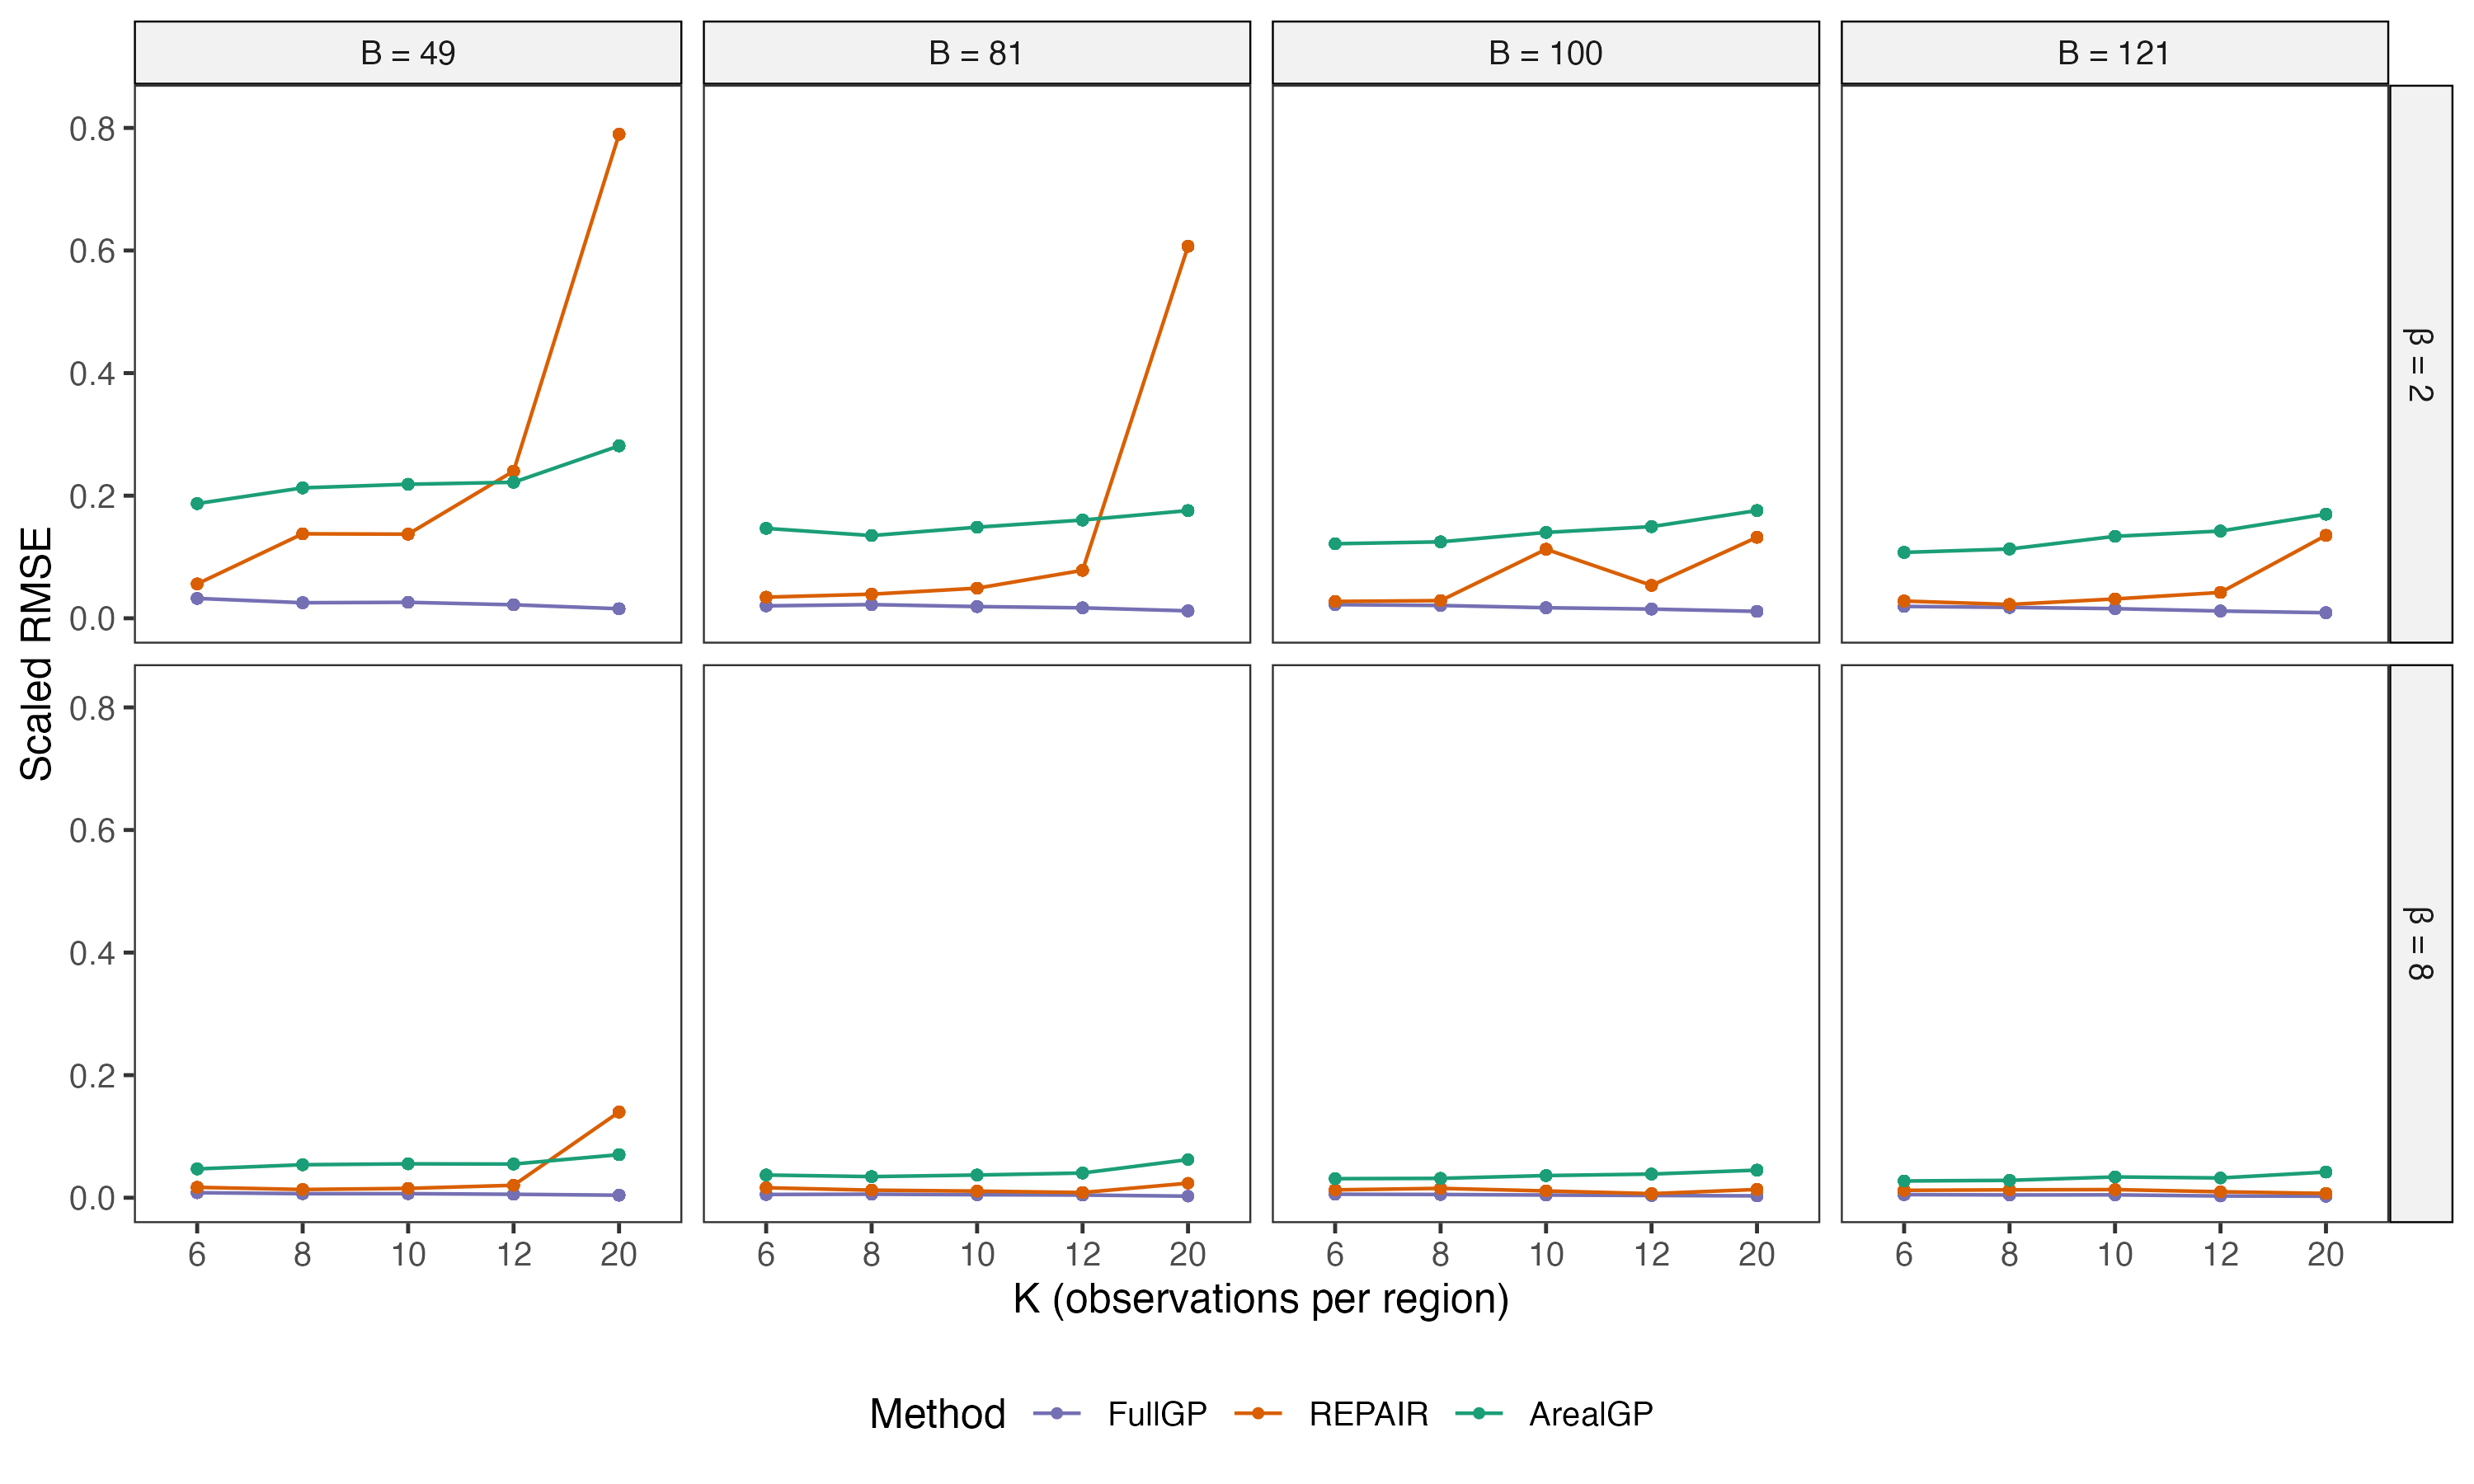
\includegraphics[width=\textwidth]{Figures/lineplot_scaled_rmse_beta.png}
    \caption{Scaled RMSE of $\hat{\beta}$ across simulation settings. Columns correspond to the number of regions $B$ and the horizontal axis shows the number of observations per region $K$. Results are reported for two SNR regimes, $\beta=2$ and $\beta=8$, comparing FullGP, ArealGP, and REPAIR.}
    \label{fig:beta_rmse_lines}
\end{figure}

Figure~\ref{fig:beta_rmse_lines} summarizes $\hat\beta$ estimation accuracy. REPAIR consistently outperforms ArealGP, with the gap widening as $B$ increases. RMSE for REPAIR rises with $K$, reflecting the harder permutation problem at larger block sizes, consistent with Theorem~\ref{thm:error-betahat}. Under high SNR ($\beta=8$), REPAIR is nearly indistinguishable from the oracle FullGP; under low SNR ($\beta=2$), the gap widens but REPAIR retains its advantage over ArealGP across most $(K,B)$ regimes. Variance and covariance parameter estimates (Figure~\ref{fig:rmse_lines} in the Supplement) show higher RMSE for REPAIR than for FullGP, consistent with the known limitations of mean-field variational approximations for nuisance covariance parameters.

Figure~\ref{fig:perm_recovery} in the Supplement reports permutation recovery. A consistent pattern is that $\bpix$ is recovered with notably higher probability than $\bpis$ across all regimes. This asymmetry is interpretable: $\bpix$ enters the likelihood directly through the signal term $\bPix\bX\beta$, so a stronger exposure signal provides more information for identifying it, while $\bpis$ affects only the latent process term $\bPis\bW$ whose recovery is governed by the spatial SNR alone. In several regimes with larger $K$, recovery of $\bpis$ degrades substantially while $\bpix$ remains well-identified. Crucially, $\beta$ estimation remains accurate throughout (Figure~\ref{fig:beta_rmse_lines}), providing direct empirical confirmation of the theoretical separation in Theorems~\ref{thm:error-pi1-pi2} and~\ref{thm:error-betahat}: consistent regression recovery does not require consistent permutation recovery.

\section{Real Data Analysis}\label{sec:data}

We illustrate REPAIR using the Meuse soil dataset \citep{pebesma2012package}, recording heavy metal concentrations and covariates at 155 locations on the river Meuse floodplain, Netherlands. We take $Y = \log(1 + \text{zinc})$ as the outcome and elevation as the exposure, center both variables, and rescale spatial coordinates to the unit square. Five observations are removed to give $n = 150$; locations are ordered by the first spatial coordinate and partitioned into contiguous blocks with exposure values and coordinates permuted within each block to induce the doubly-unlinked structure. We consider two schemes: (a) $15$ blocks of size $10$ and (b) $30$ blocks of size $5$ (Figure~\ref{fig:meuse_partition}). Full dataset background and preprocessing details are in Supplement Section~\ref{suppsec:data-details}.

\begin{figure}[t]
    \centering
    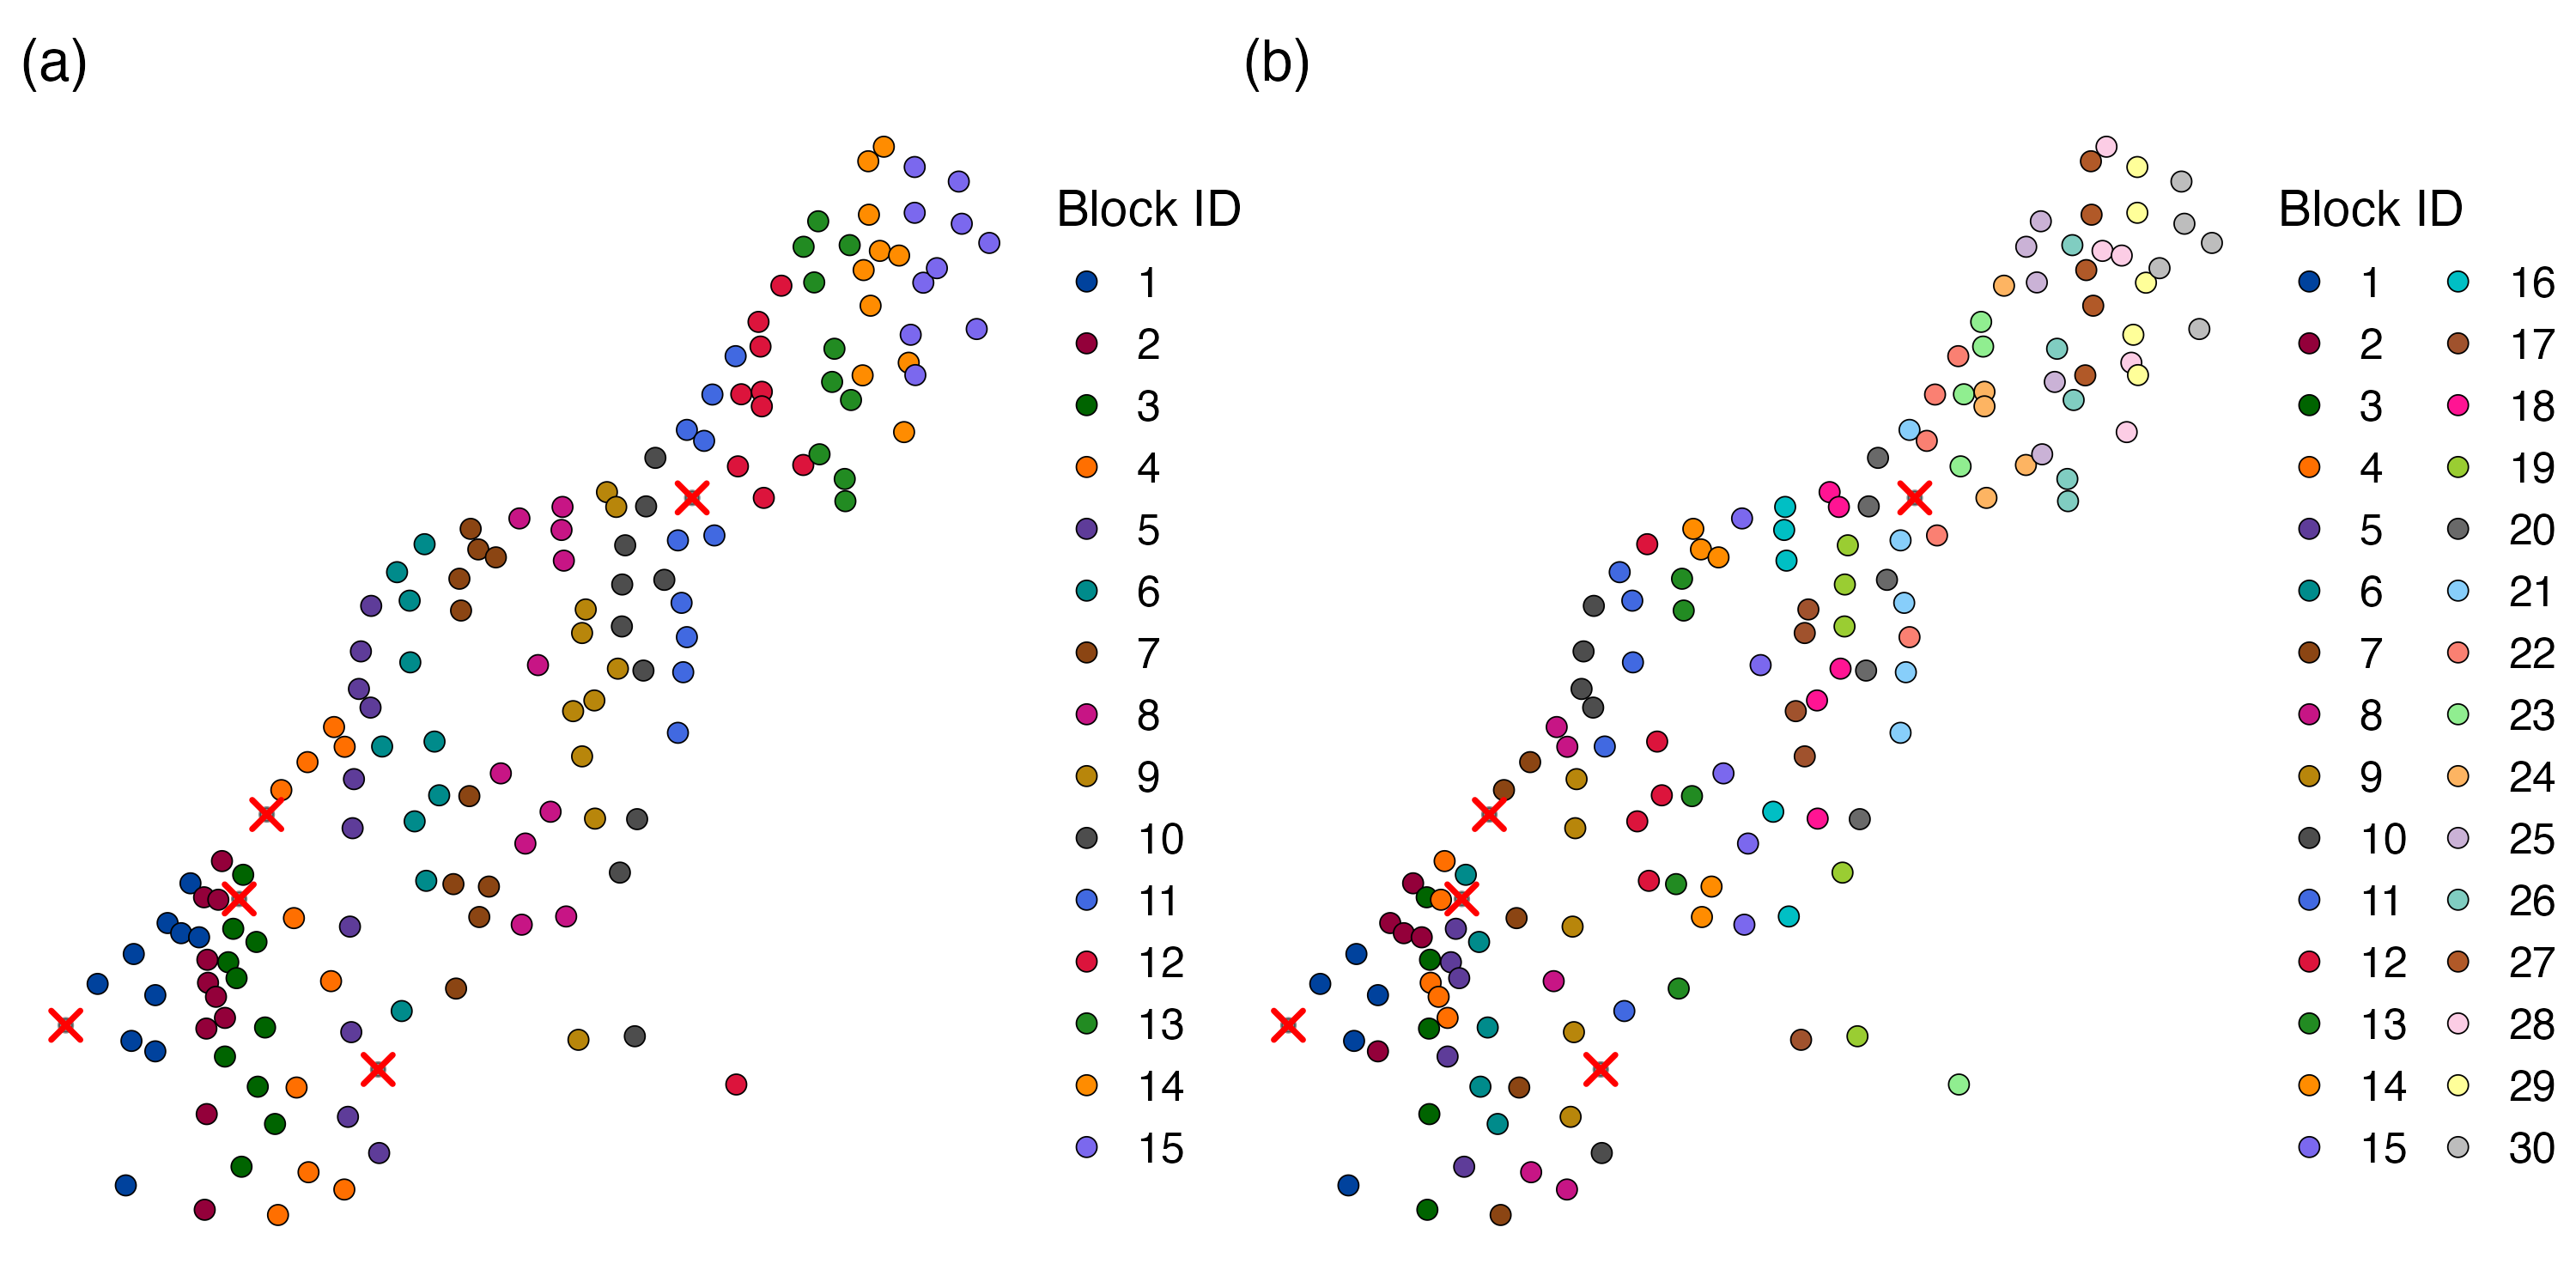
\includegraphics[width=\textwidth]{Figures/meuse_partition.png}
    \caption{Partitions for the Meuse analysis after dropping five observations: (a) $15\times 10$ and (b) $30\times 5$. Colored points denote block memberships, and red crosses indicate the removed observations.}
    \label{fig:meuse_partition}
\end{figure}

We compare \textbf{ArealGP}, \textbf{REPAIR}, and the oracle \textbf{FullGP} in effect size estimation. All three methods recover a negative effect of elevation on zinc concentration across both blocking schemes, consistent with the known pattern of higher zinc concentrations near the low-lying riverbank. The estimated regression coefficients are: $-0.2926$ (FullGP, both partitions), and under the $15\times 10$ and $30\times 5$ partitions respectively, $-0.2317$ and $-0.3965$ for ArealGP, and $-0.2102$ and $-0.2831$ for REPAIR.

Under the finer $30\times 5$ partition, REPAIR ($-0.2831$) is close to the FullGP benchmark ($-0.2926$) and outperforms ArealGP ($-0.3965$), which overshoots substantially. Under the coarser $15\times 10$ partition, where within-block permutation recovery is only partial, REPAIR ($-0.2102$) is farther from the benchmark than ArealGP ($-0.2317$); both estimates preserve the correct sign and order of magnitude. This ordering is consistent with Theorem~\ref{thm:error-betahat}: when permutation recovery degrades (large $K$, few blocks), REPAIR's advantage over a naive aggregator diminishes, yet the regression signal remains estimable.

\begin{figure}[ht]
    \centering
    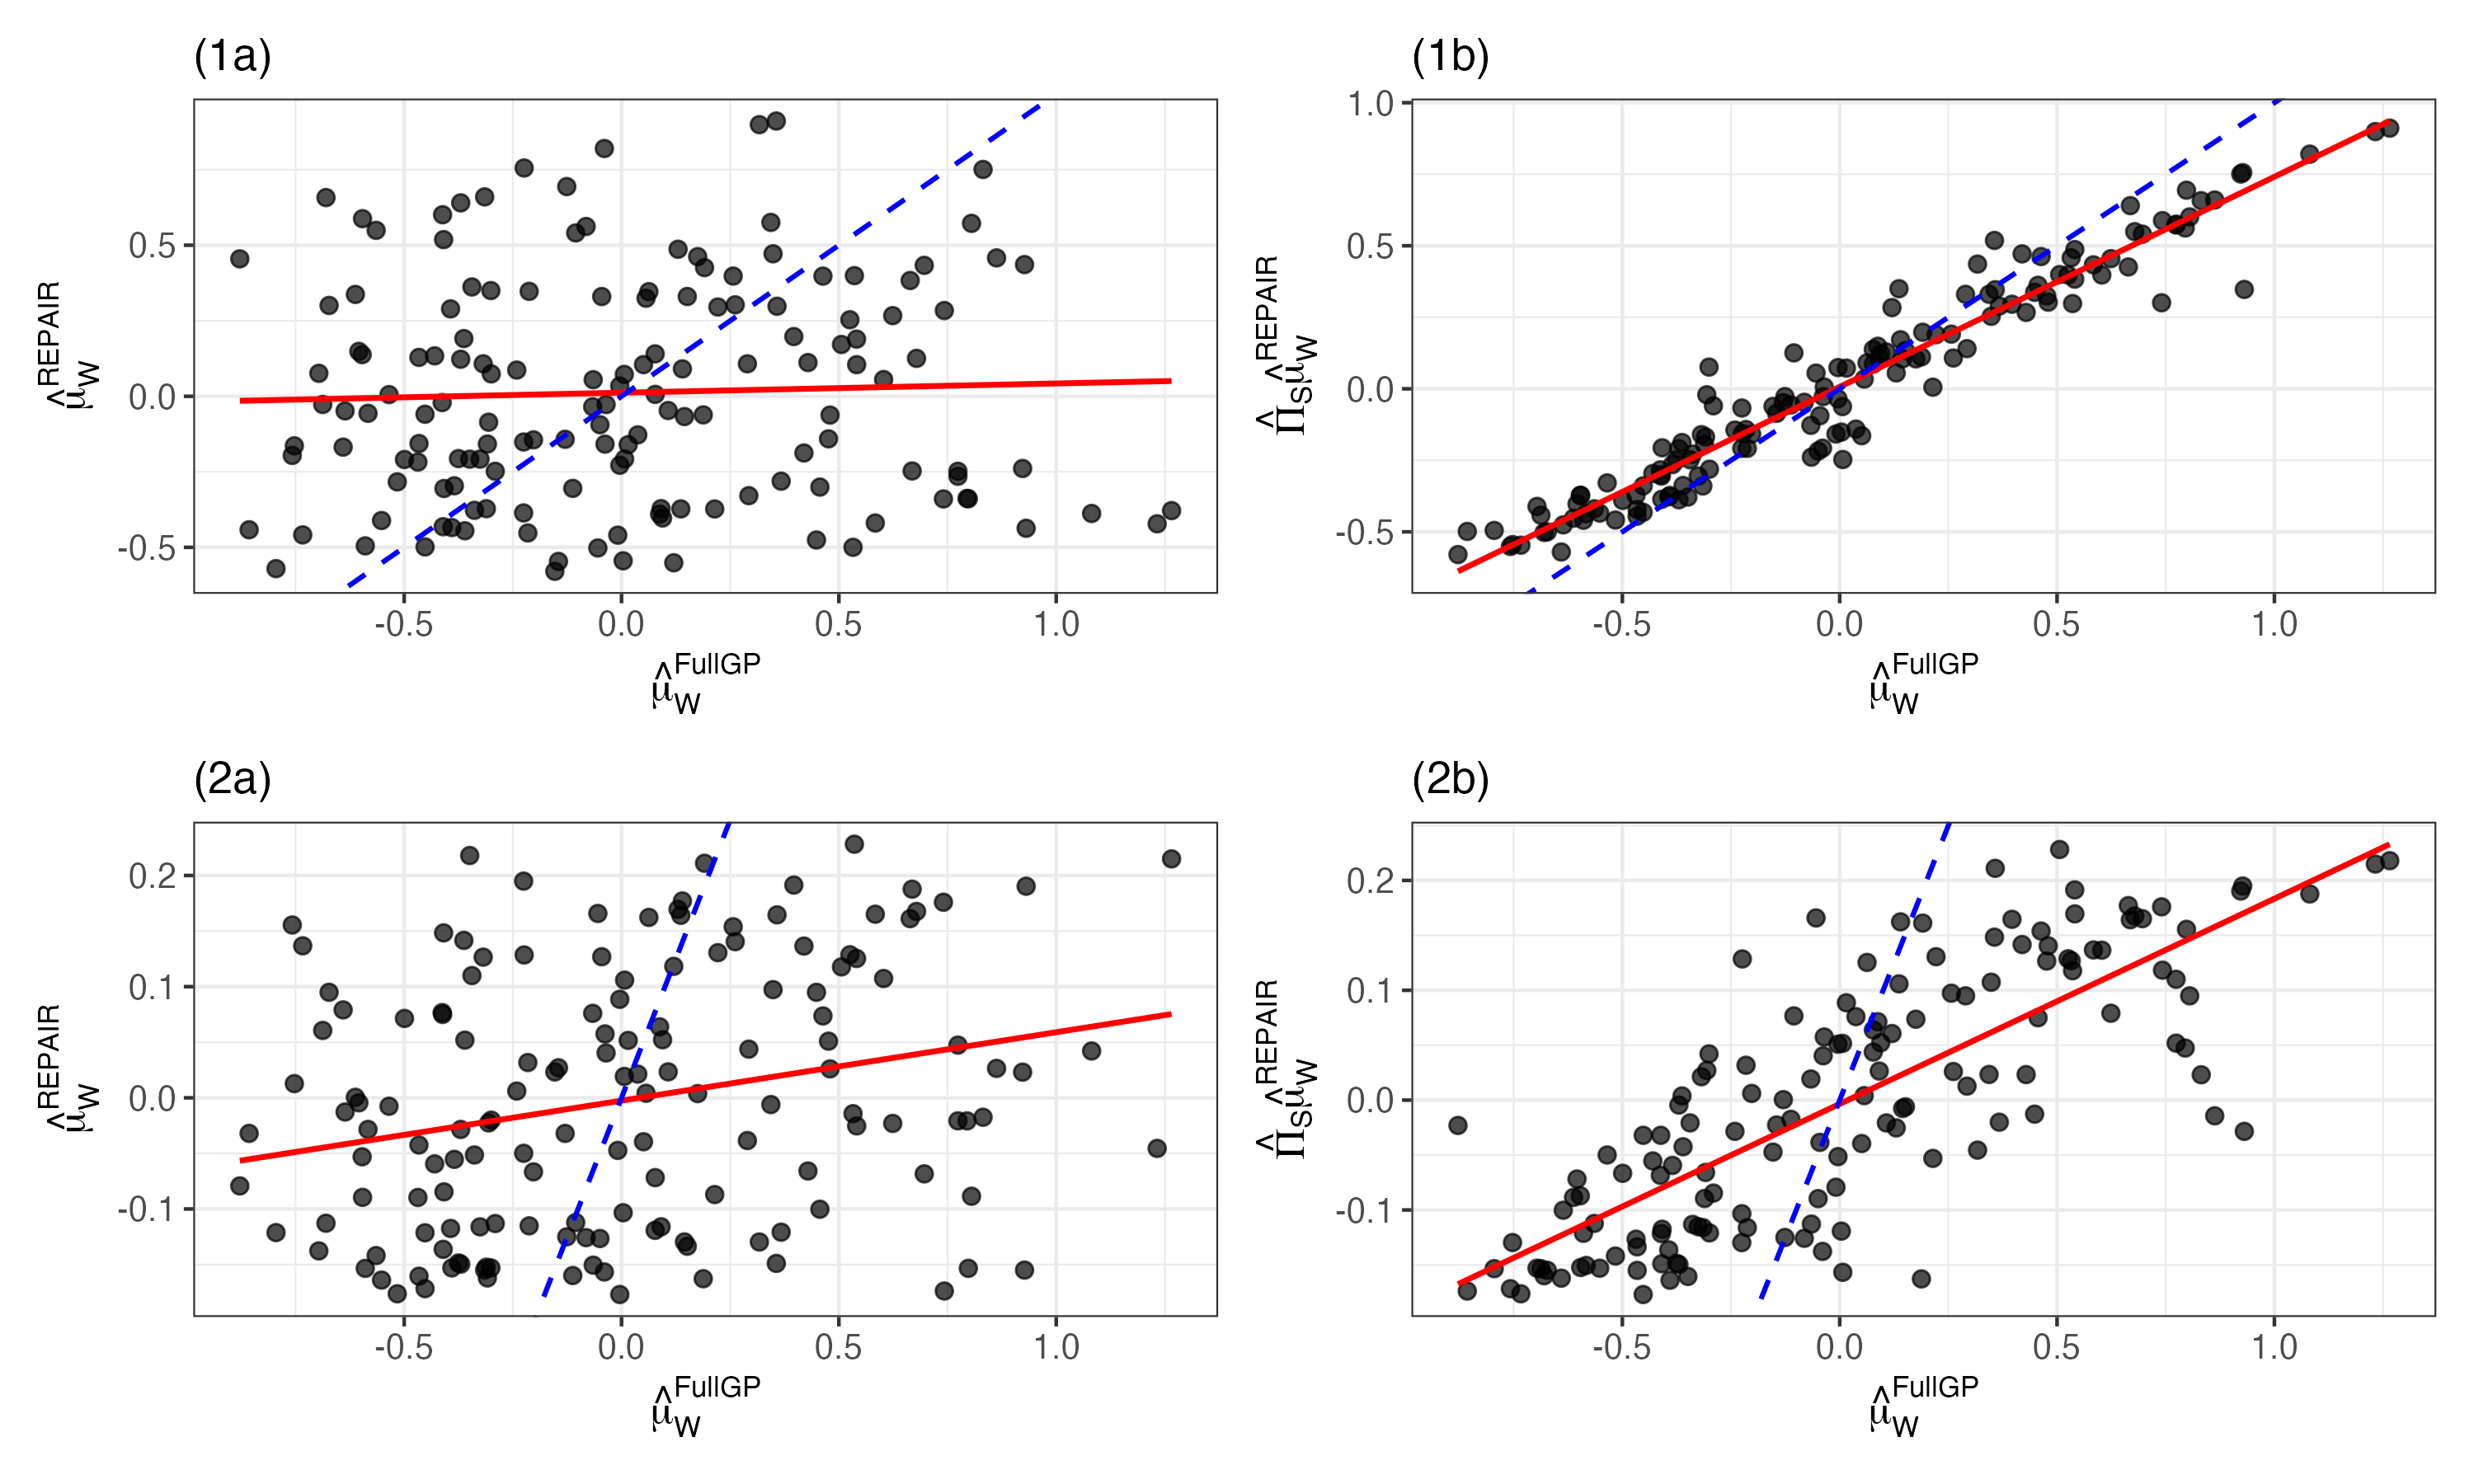
\includegraphics[width=\textwidth]{Figures/latent_surface_scatter_2by2.png}
    \caption{Comparison of latent surface estimates ($\hat{\bmu}_W$, the variational posterior mean for $\mathbb{W}_n$) from REPAIR and FullGP under the two blocking schemes. Panels (1a)--(2a) plot $\hat{\bmu}_W^{\mathrm{REPAIR}}$ against $\hat{\bmu}_W^{\mathrm{FullGP}}$; panels (1b)--(2b) plot the permutation-corrected $\widehat{\bPi}_S\hat{\bmu}_W^{\mathrm{REPAIR}}$ against $\hat{\bmu}_W^{\mathrm{FullGP}}$. Dashed blue line: $45^\circ$ reference; solid red line: least-squares fit.}
    \label{fig:latent_surface_compare}
\end{figure}

Figure~\ref{fig:latent_surface_compare} reinforces these conclusions at the level of the latent spatial surface. In the $30\times 5$ case, $\widehat{\bPi}_S\hat{\bmu}_W^{\mathrm{REPAIR}}$ aligns closely with $\hat{\bmu}_W^{\mathrm{FullGP}}$ once the estimated permutation is applied, with points lying near the $45^\circ$ line. In the $15\times 10$ case the scatter is more diffuse, reflecting partial permutation recovery. Together, the Meuse results illustrate a practically important property: REPAIR can recover the exposure effect and latent spatial surface accurately when the block structure is sufficiently fine, while even under the coarser partition the direction of the effect and a reasonable magnitude are preserved, consistent with the theoretical separation between regression and permutation recovery conditions.
\section{Discussion}\label{sec:discussion}

The central finding of this paper is that regression recovery and permutation
recovery are governed by strictly different signal-to-noise conditions in the
doubly-unlinked dependent-data setting.
The latent dependence structure provides enough information for consistent
estimation of $\beta$ even when it cannot resolve individual-level
correspondences, a separation formalised in
Theorems~\ref{thm:error-pi1-pi2} and~\ref{thm:error-betahat} that has no
counterpart in the iid shuffled regression literature
\citep{pananjady2017linear}.
Its origin lies in the covariance structure of the latent process: dependence
constrains the effective permutation space in a way that benefits regression
estimation without fully identifying the permutations themselves.

A consequence worth drawing out concerns spatial data release.
Standard geoprivacy mechanisms (spatial aggregation, noise addition) treat the tension between confidentiality and analytical
utility as fundamental, purchasing one at the cost of the other.
Our framework suggests a different possibility rooted in the Gaussian process
assumption that most spatial analyses already adopt.
Under a Gaussian process prior, individual locations are modeled as samples
from a smooth latent surface, and the scientifically relevant object is the
population-level exposure effect $\beta$, not the individual-level spatial
attribution encoded by $\bPis$.
The question our theory addresses, whether exact spatial correspondence is
necessary to recover $\beta$, follows directly from this modelling
perspective.
Theorem~\ref{thm:error-betahat} establishes that the answer is no: a
structured scrambling of both covariate assignments and spatial coordinates can
fall below the threshold sufficient for permutation recovery while leaving $\beta$
consistently estimable.
This opens the possibility of data-release mechanisms that preserve
population-level inference while masking individual-level correspondence, a
question with broad implications for spatial, temporal, and spatio-temporal
applications in environmental epidemiology, digital mental health, and spatial
transcriptomics.

Several open problems follow directly from this work.
First, establishing minimax lower bounds for the doubly-unlinked problem would
precisely characterise the information-theoretic cost of the second broken link
and determine whether the upper bounds in Theorem~\ref{thm:error-betahat} are
sharp, completing the characterisation of recovery conditions.
Second, the block structure studied here preserves coarse-scale domain ordering
while permuting within local neighbourhoods; the complementary regime, which
permutes blocks while preserving within-block structure, may better reflect
certain anonymisation or distributed data-collection mechanisms, and the
behaviour of the SNR separation in this alternative warrants separate analysis.
Third, extending the framework to multivariate exposures $\bX\in\R^p$ raises
the question of whether the separation gap between regression and permutation
recovery thresholds narrows with covariate dimension, directly relevant to
the privacy interpretation since the gap determines the strength of the
anonymisation guarantee.
Finally, the graph-indexed case, where dependence is encoded by network
structure rather than a covariance kernel, connects the doubly-unlinked regime
to the graph matching literature
\citep{arroyo2021maximum, lyzinski2014seeded, fishkind2019seeded,
dawn2025covariate} and may yield sharper recovery conditions when the graph
has known spectral properties.

\section{Data availability statement}
The data used in this study are openly available in the
Comprehensive R Archive Network (CRAN) as part of the \texttt{sp} package
\citep{pebesma2005sp} at \url{https://CRAN.R-project.org/package=sp}.
The \texttt{meuse} dataset can be loaded directly in R via
\texttt{library(sp); data(meuse)}.
The original field data were collected by \citet{rikken1993soil}.

% \if1\anon
\section{Software}
The \texttt{REPAIR} software and vignette are available at \url{https://github.com/isayantan/SpatialReg-Unlinked}.

\section{Acknowledgments}\label{sec:acknowledge}

The authors thank Dr. Debarghya Mukherjee (Department of Statistics, Boston University) for helpful discussions during the early stages of problem formulation. Portions of this research were conducted using the advanced computing resources of the Texas A\&M Department of Statistics Arseven Computing Cluster. The authors also acknowledge the use of Claude and GitHub Copilot for coding assistance and debugging, and Gemini Nano for visualization aid.

\bibliographystyle{abbrvnat}
\bibliography{doubly_unlinked}


\end{document}
